
% ----------------------------------------------------------------------
%                   LATEX TEMPLATE FOR PhD THESIS
% ----------------------------------------------------------------------

% based on Harish Bhanderi's PhD/MPhil template, then Uni Cambridge
% http://www-h.eng.cam.ac.uk/help/tpl/textprocessing/ThesisStyle/
% corrected and extended in 2007 by Jakob Suckale, then MPI-CBG PhD programme
% and made available through OpenWetWare.org - the free biology wiki


%: Style file for Latex
% Most style definitions are in the external file PhDthesisPSnPDF.
% In this template package, it can be found in ./Latex/Classes/
\documentclass[twoside,11pt]{Latex/Classes/PhDthesisPSnPDF}


%: Macro file for Latex
% Macros help you summarise frequently repeated Latex commands.
% Here, they are placed in an external file /Latex/Macros/MacroFile1.tex
% An macro that you may use frequently is the figuremacro (see introduction.tex)
\usepackage{mathtools}

\usepackage{color}

\definecolor{pblue}{rgb}{0.13,0.13,1}
\definecolor{pgreen}{rgb}{0,0.5,0}
\definecolor{pred}{rgb}{0.9,0,0}
\definecolor{pgrey}{rgb}{0.46,0.45,0.48}
\usepackage{listings}

\lstdefinestyle{customjava}{
  breakatwhitespace=false,         % sets if automatic breaks should only happen at whitespace
  breaklines=true,                 % sets automatic line breaking
  captionpos=b,                    % sets the caption-position to bottom
  extendedchars=true,              % lets you use non-ASCII characters; for 8-bits encodings only, does not work with UTF-8
  frame=single,                    % adds a frame around the code
  language=Java,                 % the language of the code
  keywordstyle=\bf,
  showspaces=false,                % show spaces everywhere adding particular underscores; it overrides 'showstringspaces'
  showstringspaces=false,          % underline spaces within strings only
  showtabs=false,                  % show tabs within strings adding particular underscores
  tabsize=2,                       % sets default tabsize to 2 spaces
  basicstyle=\footnotesize\ttfamily,
  commentstyle=\color{pgreen},
  keywordstyle=\color{pblue},
  stringstyle=\color{pred},
  moredelim=[il][\textcolor{pgrey}]{$$},
  moredelim=[is][\textcolor{pgrey}]{\%\%}{\%\%}
}

\usepackage{xcolor}
\colorlet{punct}{red!60!black}
\definecolor{background}{HTML}{EEEEEE}
\definecolor{delim}{RGB}{20,105,176}
\colorlet{numb}{magenta!60!black}

\lstdefinelanguage{json}{
    basicstyle=\normalfont\ttfamily,
    numbers=left,
    numberstyle=\scriptsize,
    stepnumber=1,
    numbersep=8pt,
    showstringspaces=false,
    breaklines=true,
    frame=lines,
    backgroundcolor=\color{background},
    literate=
     *{0}{{{\color{numb}0}}}{1}
      {1}{{{\color{numb}1}}}{1}
      {2}{{{\color{numb}2}}}{1}
      {3}{{{\color{numb}3}}}{1}
      {4}{{{\color{numb}4}}}{1}
      {5}{{{\color{numb}5}}}{1}
      {6}{{{\color{numb}6}}}{1}
      {7}{{{\color{numb}7}}}{1}
      {8}{{{\color{numb}8}}}{1}
      {9}{{{\color{numb}9}}}{1}
      {:}{{{\color{punct}{:}}}}{1}
      {,}{{{\color{punct}{,}}}}{1}
      {\{}{{{\color{delim}{\{}}}}{1}
      {\}}{{{\color{delim}{\}}}}}{1}
      {[}{{{\color{delim}{[}}}}{1}
      {]}{{{\color{delim}{]}}}}{1},
}

% This file contains macros that can be called up from connected TeX files
% It helps to summarise repeated code, e.g. figure insertion (see below).

% insert a centered figure with caption and description
% parameters 1:filename, 2:title, 3:description and label
\newcommand{\figuremacro}[3]{
	\begin{figure}[htbp]
		\centering
		\includegraphics[width=1\textwidth]{#1}
		\caption[#2]{\textbf{#2} - #3}
		\label{#1}
	\end{figure}
}

% insert a centered figure with caption and description AND WIDTH
% parameters 1:filename, 2:title, 3:description and label, 4: textwidth
% textwidth 1 means as text, 0.5 means half the width of the text
\newcommand{\figuremacroW}[4]{
	\begin{figure}[htbp]
		\centering
		\includegraphics[width=#4\textwidth]{#1}
		\caption[#2]{\textbf{#2} - #3}
		\label{#1}
	\end{figure}
}

% inserts a figure with wrapped around text; only suitable for NARROW figs
% o is for outside on a double paged document; others: l, r, i(inside)
% text and figure will each be half of the document width
% note: long captions often crash with adjacent content; take care
% in general: above 2 macro produce more reliable layout
\newcommand{\figuremacroN}[3]{
	\begin{wrapfigure}{o}{0.5\textwidth}
		\centering
		\includegraphics[width=0.48\textwidth]{#1}
		\caption[#2]{{\small\textbf{#2} - #3}}
		\label{#1}
	\end{wrapfigure}
}

% predefined commands by Harish
\newcommand{\PdfPsText}[2]{
  \ifpdf
     #1
  \else
     #2
  \fi
}

\newcommand{\IncludeGraphicsH}[3]{
  \PdfPsText{\includegraphics[height=#2]{#1}}{\includegraphics[bb = #3, height=#2]{#1}}
}

\newcommand{\IncludeGraphicsW}[3]{
  \PdfPsText{\includegraphics[width=#2]{#1}}{\includegraphics[bb = #3, width=#2]{#1}}
}

\newcommand{\InsertFig}[3]{
  \begin{figure}[!htbp]
    \begin{center}
      \leavevmode
      #1
      \caption{#2}
      \label{#3}
    \end{center}
  \end{figure}
}


%%% Local Variables: 
%%% mode: latex
%%% TeX-master: "~/Documents/LaTeX/CUEDThesisPSnPDF/thesis"
%%% End: 




%: ----------------------------------------------------------------------
%:                  TITLE PAGE: name, degree,..
% ----------------------------------------------------------------------
% below is to generate the title page with crest and author name

%if output to PDF then put the following in PDF header
\ifpdf  
    \pdfinfo { /Title  (Enhancing 3D reconstruction with Mobile Sensors Data)
               /Creator (TeX)
               /Producer (pdfTeX)
               /Author (Krzysztof Wróbel krzysztof@velocicaptor.com)
               /CreationDate (D:YYYYMMDDhhmmss)  %format D:YYYYMMDDhhmmss
               /ModDate (D:YYYYMMDDhhmm)
               /Subject (xyz)
               /Keywords (3D reconstruction, Augmented Relaity, AR, Sensor, Accelerometer, Gyroscope, Sensor Fusion, Bundle Adjustment, Pose Estimation) }
    \pdfcatalog { /PageMode (/UseOutlines)
                  /OpenAction (fitbh)  }
\fi

%% Titeseite

\begin{titlepage}
  \begin{center}
	  
    %\mbox{}

    %\vspace{1cm}

	\centering
	
\includegraphics[width=3cm]{figures/tub.pdf}\\
	\vspace{0.8em}
	\LARGE 

	\textsc{Technische Universit\"at Berlin}

    \vspace{1cm}

    \sffamily \LARGE \textbf{My new Master thesis titel comes here}

    \vspace{1.5cm}





    \normalsize vorgelegt von

    \vspace{.1cm}

    \large Alex the student (Dipl.-Ing.)

    \vspace{.8cm}

  %  von der Fakult�t IV - Elektrotechnik und Informatik der Technischen Universit�t Berlin


    \normalsize von der Fakult\"{a}t IV -- Elektrotechnik und Informatik\\
    %\vspace{.1cm}
    \normalsize der Technischen Universit\"{a}t Berlin\\
    %\vspace{.1cm}
    \normalsize zur Erlangung des akademischen Grades\\
    %\vspace{.1cm}
    \large \textsc{Diplom der Ingenieurwissenschaften (Dipl.-Ing.)}\\
    %\vspace{.1cm}
    \normalsize genemigte Diplomarbeit\\

    \vspace{1cm}

    \large \textbf{Diplomausschuss:}

    \vspace{.2cm}

		\begin{tabular}{rl}
		Pr\"ufer der Diplomarbeit:	& Prof. Dr.-Ing. XYZ, TU-Berlin\\
						& Dr.-Ing. XYZ, TU-Berlin\\
		\end{tabular}\\

    \vspace{2cm}
    \large Tag der wissenschaftlichen Verteidigung: 11.01.2013\\
    \vspace{0.5cm}
    \large Berlin 2013\\

  \end{center}
\end{titlepage}


\title{Enhancing 3D reconstruction using Mobile Sensors Data}



% ----------------------------------------------------------------------
% The section below defines www links/email for author and institutions
% They will appear on the title page of the PDF and can be clicked
\ifpdf
  \author{\href{mailto:krzysztof@velocicaptor.com}{Krzysztof Wróbel}}
%  \cityofbirth{born in XYZ} % uncomment this if your university requires this
%  % If city of birth is required, also uncomment 2 sections in PhDthesisPSnPDF
%  % Just search for the "city" and you'll find them. TODO
  \collegeordept{\href{http://www.something.net}{CollegeOrDepartment}}
  \university{\href{http://www.something.net}{University}}

  % The crest is a graphics file of the logo of your research institution.
  % Place it in ./0_frontmatter/figures and specify the width
  \crest{
\includegraphics[width=4cm]{logo}}
  
% If you are not creating a PDF then use the following. The default is PDF.
\else
  \author{Krzysztof Wróbel}
%  \cityofbirth{born in XYZ}
  \collegeordept{CollegeOrDept}
  \university{University}
  \crest{
\includegraphics[width=4cm]{logo}}
\fi

%\renewcommand{\submittedtext}{change the default text here if needed}
\degree{Philosophi\ae Doctor (PhD), DPhil,..}
\degreedate{year month}


% ----------------------------------------------------------------------
       
% turn of those nasty overfull and underfull hboxes
\hbadness=10000
\hfuzz=50pt


%: --------------------------------------------------------------
%:                  FRONT MATTER: dedications, abstract,..
% --------------------------------------------------------------

\begin{document}

%\language{english}

% sets line spacing
\renewcommand\baselinestretch{1.2}
\baselineskip=18pt plus1pt


%: ----------------------- generate cover page ------------------------

\maketitle  % command to print the title page with above variables


%: ----------------------- cover page back side ------------------------
% Your research institution may require reviewer names, etc.
% This cover back side is required by Dresden Med Fac; uncomment if needed.

\newpage
\vspace{10mm}
1. Reviewer: Name

\vspace{10mm}
2. Reviewer: 

\vspace{20mm}
Day of the defense:

\vspace{20mm}
\hspace{70mm}Signature from head of PhD committee:



%: ----------------------- abstract ------------------------

% Your institution may have specific regulations if you need an abstract and where it is to be placed in the document. The default here is just after title.


% Thesis Abstracts -----------------------------------------------------

\selectlanguage{english}
\begin{abstract}
The main subject of this thesis addresses the possibility of enhancing the existing 3D reconstruction algorithms with additional Android sensor fusion data. The primary fundamentals behind the reconstruction techniques and the problems related to them are explained in order to introduce the reader to these topics. Related works are discussed in order to explain the strengths and weaknesses of the state-of-art reconstruction approches. The proposed enhancements using initial rotation in the standard 8-point and 5-point algorithms are explained in detail. Both of them allow for focusing on correcting rotation matrix error instead of calculating the rotation itself. This, in turn, serves for reducing ambiguity of the decomposition of essential matrix to the relative rotation and translation of the cameras. The primary idea behind the implementation of the 3-point algorithm for translation is also described. The most important aspects of the implemented $"Sensor Enhanced Image Camera"$ Android application and $"Enhanced 3D Reconstructer"$ were discussed.
The three proposed initial pair reconstruction methods were evaluated, which showed that each algorithm is able to improve certain asspects of the 3D reconstruction. Different reconstruction strategies were evaluated. As a result it was discovered that the enhanced structure computation can be faster and more accurate than the standard methodology. Using initial rotation and translation pose estimation results in significantly faster convergence and better error reduction with Bundle Adjustment. This thesis covers only some notions of the Structure from Motion, therefore plans for future development were  established.
\end{abstract}

\clearpage
\selectlanguage{ngerman} 
\begin{abstract}
Das Hauptthema dieser Arbeit befasst sich mit der M{\"o}glichkeit der Verbesserung der vorhandenen 3D-Rekonstruktionsalgorithmen mit zus{\"a}tzlichen Android Sensorfusion Daten. Die wichtigsten Grundlagen hinter den Rekonstruktionstechniken und die damit verbundenen Probleme sind, um den Leser zu diesen Themen vorstellen erl{\"a}utert. {\"A}hnliche Arbeiten sind erforderlich, um die Festigkeiten und Schw{\"a}chen der Stand-der-Technik Rekonstruktion Ansätze erkl{\"a}ren diskutiert. Die vorgeschlagenen Verbesserungen mit Anfangsrotation in den Standard 8-Punkte und 5-Punkte-Algorithmen werden im Detail erkl{\"a}rt. Beide von ihnen k{\"o}nnen zur Fokussierung auf die Rotationsmatrix Fehler Korrektur anstelle der Berechnung des Rotation selbst. Dies wiederum serviert zur Reduzierung der Mehrdeutigkeit des Essential-Matrix Zersetzungs zu der relativen Rotation und Translation den Kameras. Die Hauptidee hinter der Umsetzung der 3-Punkt-Algorithmus f{\"u}r die Translation ist ebenfalls beschrieben. Die wichtigsten Aspekte die implementierten $"Sensor Verbesserte Bildkamera "$ Android-Anwendung und $ "Verbesserte 3D Reconstructer "$  wurden diskutiert.
Die drei vorgeschlagenen ersten Paar Rekonstruktionsmethoden wurden bewertet, die zeigten, dass jeder Algorithmus kann bestimmte asspects der 3D-Rekonstruktion zu verbessern. Verschiedene Rekonstruktionsstrategien wurden bewertet. Als Ergebnis wurde festgestellt, dass die verbesserte Struktur Berechnung kann schneller und genauer als die Standardmethode sein. Mit  anfänglichen Rotation und Translation  Posenschätzung resultiert in signifikant schneller Konvergenz und besseres Fehlerreduktion mit B{\"u}ndelausgleichung. Diese Diplomarbeit umfasst nur einige Vorstellungen von der Struktur aus Bewegung, daher plant f{\"u}r die zuk{\"u}nftige Entwicklung entstanden.
\end{abstract}
\selectlanguage{english}

% The original template provides and abstractseparate environment, if your institution requires them to be separate. I think it's easier to print the abstract from the complete thesis by restricting printing to the relevant page.
% \begin{abstractseparate}
%   
% Thesis Abstracts -----------------------------------------------------

\selectlanguage{english}
\begin{abstract}
The main subject of this thesis addresses the possibility of enhancing the existing 3D reconstruction algorithms with additional Android sensor fusion data. The primary fundamentals behind the reconstruction techniques and the problems related to them are explained in order to introduce the reader to these topics. Related works are discussed in order to explain the strengths and weaknesses of the state-of-art reconstruction approches. The proposed enhancements using initial rotation in the standard 8-point and 5-point algorithms are explained in detail. Both of them allow for focusing on correcting rotation matrix error instead of calculating the rotation itself. This, in turn, serves for reducing ambiguity of the decomposition of essential matrix to the relative rotation and translation of the cameras. The primary idea behind the implementation of the 3-point algorithm for translation is also described. The most important aspects of the implemented $"Sensor Enhanced Image Camera"$ Android application and $"Enhanced 3D Reconstructer"$ were discussed.
The three proposed initial pair reconstruction methods were evaluated, which showed that each algorithm is able to improve certain asspects of the 3D reconstruction. Different reconstruction strategies were evaluated. As a result it was discovered that the enhanced structure computation can be faster and more accurate than the standard methodology. Using initial rotation and translation pose estimation results in significantly faster convergence and better error reduction with Bundle Adjustment. This thesis covers only some notions of the Structure from Motion, therefore plans for future development were  established.
\end{abstract}

\clearpage
\selectlanguage{ngerman} 
\begin{abstract}
Das Hauptthema dieser Arbeit befasst sich mit der M{\"o}glichkeit der Verbesserung der vorhandenen 3D-Rekonstruktionsalgorithmen mit zus{\"a}tzlichen Android Sensorfusion Daten. Die wichtigsten Grundlagen hinter den Rekonstruktionstechniken und die damit verbundenen Probleme sind, um den Leser zu diesen Themen vorstellen erl{\"a}utert. {\"A}hnliche Arbeiten sind erforderlich, um die Festigkeiten und Schw{\"a}chen der Stand-der-Technik Rekonstruktion Ansätze erkl{\"a}ren diskutiert. Die vorgeschlagenen Verbesserungen mit Anfangsrotation in den Standard 8-Punkte und 5-Punkte-Algorithmen werden im Detail erkl{\"a}rt. Beide von ihnen k{\"o}nnen zur Fokussierung auf die Rotationsmatrix Fehler Korrektur anstelle der Berechnung des Rotation selbst. Dies wiederum serviert zur Reduzierung der Mehrdeutigkeit des Essential-Matrix Zersetzungs zu der relativen Rotation und Translation den Kameras. Die Hauptidee hinter der Umsetzung der 3-Punkt-Algorithmus f{\"u}r die Translation ist ebenfalls beschrieben. Die wichtigsten Aspekte die implementierten $"Sensor Verbesserte Bildkamera "$ Android-Anwendung und $ "Verbesserte 3D Reconstructer "$  wurden diskutiert.
Die drei vorgeschlagenen ersten Paar Rekonstruktionsmethoden wurden bewertet, die zeigten, dass jeder Algorithmus kann bestimmte asspects der 3D-Rekonstruktion zu verbessern. Verschiedene Rekonstruktionsstrategien wurden bewertet. Als Ergebnis wurde festgestellt, dass die verbesserte Struktur Berechnung kann schneller und genauer als die Standardmethode sein. Mit  anfänglichen Rotation und Translation  Posenschätzung resultiert in signifikant schneller Konvergenz und besseres Fehlerreduktion mit B{\"u}ndelausgleichung. Diese Diplomarbeit umfasst nur einige Vorstellungen von der Struktur aus Bewegung, daher plant f{\"u}r die zuk{\"u}nftige Entwicklung entstanden.
\end{abstract}
\selectlanguage{english}
% \end{abstractseparate}


%: ----------------------- tie in front matter ------------------------

\frontmatter
% Thesis Dedictation ---------------------------------------------------
% ----------------------------------------------------------------------
% Thesis Acknowledgements ------------------------------------------------


%\begin{acknowledgementslong} %uncommenting this line, gives a different acknowledgements heading
\begin{acknowledgements}      %this creates the heading for the acknowlegments

I would like to acknowledge the thousands of individuals who have coded for the LaTeX project for free. It is due to their efforts that we can generate professionally typeset PDFs now.

\end{acknowledgements}
%\end{acknowledgmentslong}

% ------------------------------------------------------------------------





%: ----------------------- contents ------------------------

\setcounter{secnumdepth}{3} % organisational level that receives a numbers
\setcounter{tocdepth}{3}    % print table of contents for level 3
\tableofcontents            % print the table of contents
% levels are: 0 - chapter, 1 - section, 2 - subsection, 3 - subsection


%: ----------------------- list of figures/tables ------------------------

\listoffigures	% print list of figures

\listoftables  % print list of tables


%: ----------------------- glossary ------------------------

% Tie in external source file for definitions: /0_frontmatter/glossary.tex
% Glossary entries can also be defined in the main text. See glossary.tex
% this file is called up by thesis.tex
% content in this file will be fed into the main document

% Glossary entries are defined with the command \nomenclature{1}{2}
% 1 = Entry name, e.g. abbreviation; 2 = Explanation
% You can place all explanations in this separate file or declare them in the middle of the text. Either way they will be collected in the glossary.

% required to print nomenclature name to page header
\markboth{\MakeUppercase{\nomname}}{\MakeUppercase{\nomname}}


% ----------------------- contents from here ------------------------

%% chemicals
%\nomenclature{DAPI}{4',6-diamidino-2-phenylindole; a fluorescent stain that binds strongly to DNA and serves to marks the nucleus in fluorescence microscopy} 
%\nomenclature{DEPC}{diethyl-pyro-carbonate; used to remove RNA-degrading enzymes (RNAases) from water and laboratory utensils}
%\nomenclature{DMSO}{dimethyl sulfoxide; organic solvent, readily passes through skin, cryoprotectant in cell culture}
%\nomenclature{EDTA}{Ethylene-diamine-tetraacetic acid; a chelating (two-pronged) molecule used to sequester most divalent (or trivalent) metal ions, such as calcium (Ca$^{2+}$) and magnesium (Mg$^{2+}$), copper (Cu$^{2+}$), or iron (Fe$^{2+}$ / Fe$^{3+}$)}



 

\begin{multicols}{2} % \begin{multicols}{#columns}[header text][space]
\begin{footnotesize} % scriptsize(7) < footnotesize(8) < small (9) < normal (10)

\printnomenclature[1.5cm] % [] = distance between entry and description
\label{nom} % target name for links to glossary

\end{footnotesize}
\end{multicols}



%: --------------------------------------------------------------
%:                  MAIN DOCUMENT SECTION
% --------------------------------------------------------------

% the main text starts here with the introduction, 1st chapter,...
\mainmatter

\renewcommand{\chaptername}{} % uncomment to print only "1" not "Chapter 1"


%: ----------------------- subdocuments ------------------------

% Parts of the thesis are included below. Rename the files as required.
% But take care that the paths match. You can also change the order of appearance by moving the include commands.

% this file is called up by thesis.tex
% content in this file will be fed into the main document

%: ----------------------- introduction file header -----------------------
\chapter{Introduction}
% the code below specifies where the figures are stored
\ifpdf
    \graphicspath{{1_introduction/figures/PNG/}{1_introduction/figures/PDF/}{1_introduction/figures/}}
\else
    \graphicspath{{1_introduction/figures/EPS/}{1_introduction/figures/}}
\fi

% ----------------------------------------------------------------------
%: ----------------------- introduction content ----------------------- 
% ----------------------------------------------------------------------

Mobile and wearable devices are becoming more and more popular. Modern smartphones despite having extremely good camera's also use advanced sensor's, like accelerometers, gyroscope, magnetometer, barometer etc.. There is also a big need and growing market of Augmented Reality (AR) and Virtual Reality(VR). That is why image analysis and recognition, as well as 3-D reconstruction techniques are really hot topic. Unfortunately algorithms that support these techniques are very time and memory consuming, that is why it is really hard to run them on mobile devices, which have many limitations in terms of CPU speed and RAM memory capacity.

\section{Purpose of this thesis} % section headings are printed smaller than chapter names
Author of this document will present the reader with an overview of the idea of 3D reconstruction techniques. This thesis also inculdes brief description of related research conducted in this area. After short analysis of efficiency, accuracy and common problems of few chosen algorithms this thesis will propose their enhacment using data acquired from Android sensor fusion. Two application was created in order to verify and test proposed algorithms and reconstruction strategies. Both Android and Desktop applications will be discussed in important implementation asspects. This thesis also explains the reader meaning of testing results. At the end conclusions and encountered errors are discussed. Finally futur plans for conducted research is presented.
\section{Scope}
The author researched, how fusion of accelerometer, gyroscope and magnetometer can be used in order to improve fundamental, essential matrix calculations and also relative pose estimation. Unfortunately raw data sensors are really noisy and therefore not reliable enough to relay solely on them to enhance reconstruction. Heuristic measurment of translation used for enhancment using linear-acceleration was also concepted and implemented by author. In this research introduced are  initial rotation enhanced 8-point and 5-point reconstruction algorithms. Also alternative 3-point algorithm for translation estimation is also discussed and implemented.
This thesis deals only with initial pair images reconstruction and relative pose estimation for Structure from Motion computation. It is not researched, what are the best methodology for corresponding feature computation, but other possibilities of point matching are discussed. Finally it is reserched, how improved versions of standard 8-point and 5-point algorithms influence convergence speed and error reduction of Bundle Adjustment.
\section{Initial assumptions}
The general process of 3-D reconstruction is quite broad, that's why the author of the thesis focus only on certain aspects of this topic. That is why author did not write all algorithms from the scratch, but built his versions on top of OpenCV library and open-source project called "Relative Pose Esitmation" created by TODO . In terms of sensor fusion, currently state of art approach can be found on Android platform. 3D reconstruction process will be processed in seperate desktop application.
\section{Thesis Outline}
In \textbf{Chapter 2} fundamental technology behind 3D reconstruction and Structure from Motion was discussed. Also sensors used to perform sensor fusion on Android platform were briefly introduced.
\\*
In \textbf{Chapter 3} brief overview of related research was made. Most interesting discoveries, which lead to conception of proposed methods were also described. 
\\*
In \textbf{Chapter 4} teoretical concept of proposed 8-point and 5-point rotation enhanced algorithms were presented. Also alternative approach to 3-point translation estimation was made. Finally author proposed few most promising Structure from motion reconstruction strategies.
\\*
In \textbf{Chapter 5} most important implementation asspects of rotation and translation measurements were discussed. Also enhancements modifications to standard 8-point and 5-point algorithms were discussed. Also 3-point translation estimation approach and relative pose ehancements implementation was discussed.
\\*
In \textbf{Chapter 6} evaluation of proposed initial pair reconstruction methods and strategies was presented and discussed.
\\*
In \textbf{Chapter 7} conslusions observed during master thesis project period, as well as encounterd problems were discussed. Thesis ends with further development plans establishment.

% ----------------------------------------------------------------------



	% background information
% this file is called up by thesis.tex
% content in this file will be fed into the main document

\chapter{Fundamentals} % top level followed by section, subsection
This chapter explains the basic theory of 3D reconstruction and Structure from Motion. All information referred to herein can be found in \cite{HartleyMultipleView}. It also includes brief overview of sensor fusion made with the use of accelerometer, gyroscope and magnetometer data. 

% ----------------------- contents from here ------------------------
\section{3-D reconstruction in general}
There are many possibilities of performing reconstruction, starting from two-view reconstruction, multiple-view reconstruction and ending with the use of stereo calibrated cameras like the ones used in Kinect[reference]. Reconstruction can also be performed with a single hand-held camera either from a video or a sequence of images. As little as two pictures taken from different angles of a single object are sufficient to perform 3D model generation. Reconstruction process consists of the following steps:
\setlist[2]{noitemsep} % sets the itemsep and parsep for all level two lists to 0
\setenumerate{noitemsep} % sets no itemsep for enumerate lists only
\begin{enumerate}
\item \textbf{Image Acquistion}, where images are acquired 
\item \textbf{Feature extraction and corresponding points matching}, where distinctive features are extracted from the images and compared
\item \textbf{Fundamental \& Essential Matrices}, where matrices meeting the requirements of basic epipolar geometry are calculated
\item \textbf{Camera parameters estimation}, where external and internal camera parameters are estimated
\item \textbf{Triangulation}, where camera projection matrices are composed and used in order to calculate 3D cloud points
\end{enumerate}
\subsection{Feature extraction and corresponding points matching}
Usually, each image used in reconstruction has to be analysed in order for the dstinctive features to be found. Afterwards all features in images are compared in order to find corresponding matches(\ref{fig:correspondingMatches}).
\begin{figure}[p]
    \centering
    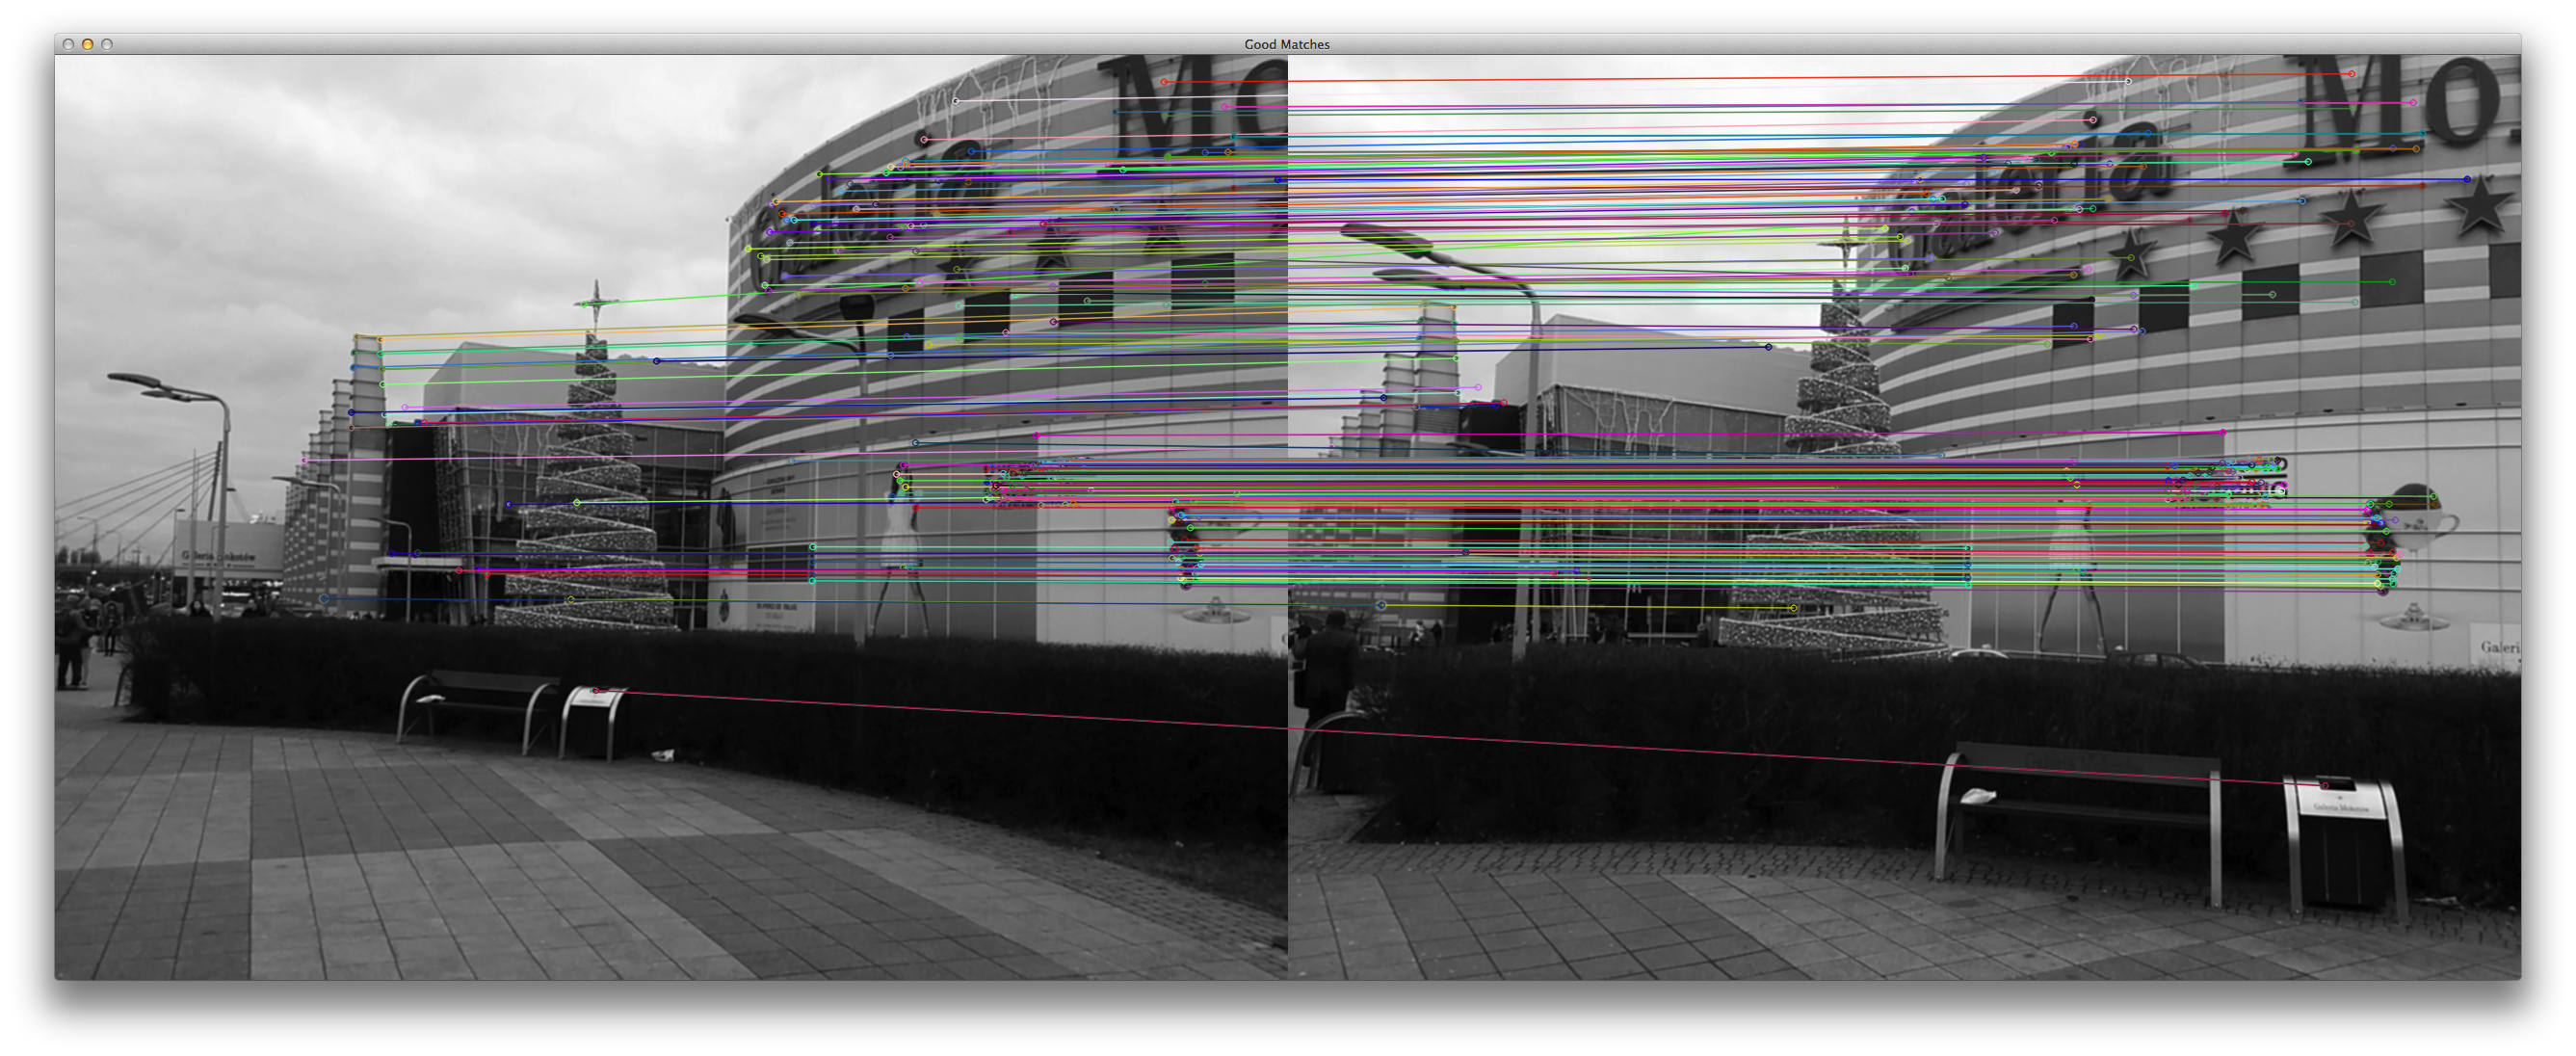
\includegraphics[width=0.8\textwidth]{correspondingMatching}
    \caption{}
    \label{fig:correspondingMatches}
\end{figure}
There are multiple features detectors and extractors available for use \url{$http://en.wikipedia.org/wiki/Feature_detection_%28computer_vision%29$}. Some of them are more suitable for edge detection, while others are best used for corner or blob detection. One of the most popluar and robust feature detection method is scale-invariant feature transform (SIFT) \url{http://en.wikipedia.org/wiki/Scale-invariant_feature_transform}. The use of these descriptors allows for detecting local features in images and describing them with metrics including scale, rotation and translation invariant.
\subsection{Fundamental \& Essential Matrix estimations}
Once proper matches are found, it can be proven that there exsists Fundamental matrix F for which the following equation is satisfied:
\begin{equation} \label{eq:fundamntalEquation}
{x}^{'T} * F * x = 0
\end{equation} 
where $x$ and ${x}_{'}$ are uncalibrated notions of points correspondence \cite{HartletMultipleView}TODO chapter. It is known that soultuions of this equation are highly sensitive to the occurence of outliers. Usually, to make fundamental matrix estimations more accurate some outliers removing algorithms need to be used. One of the most robust approaches includes the use of of RANdom SAmple Consensus (\gls{ransac}) \url{http://en.wikipedia.org/wiki/RANSAC}. The example of sample fitting can be seen in \ref{fig:RANSACFitting}
\begin{figure}[p]
    \centering
    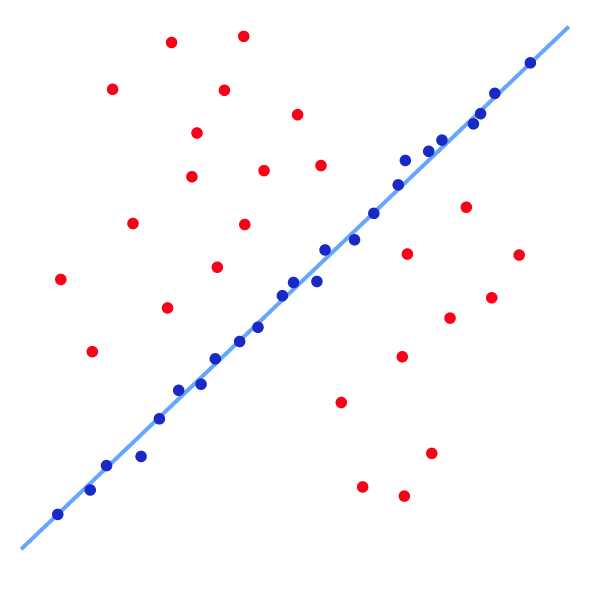
\includegraphics[width=0.8\textwidth]{RANSACFitting}
    \caption{RANSAC fitting for 2D image TODO reference}
    \label{fig:RANSACFitting}
\end{figure}
Its basic idea relies on choosing a random subset from among all matches, solving a problem of reduced dataset and establishing how many points from the original set satisfy the equation.
The use of F matrix allows for calculating epipolar lines for each point (\ref{fig:EpipolarGeometry}). These lines cross exactly the same points in both images and can be used for dense feature matching sinces matches need to be searched for exclusively in the surroundings of these lines.
\begin{figure}[p]
    \centering
    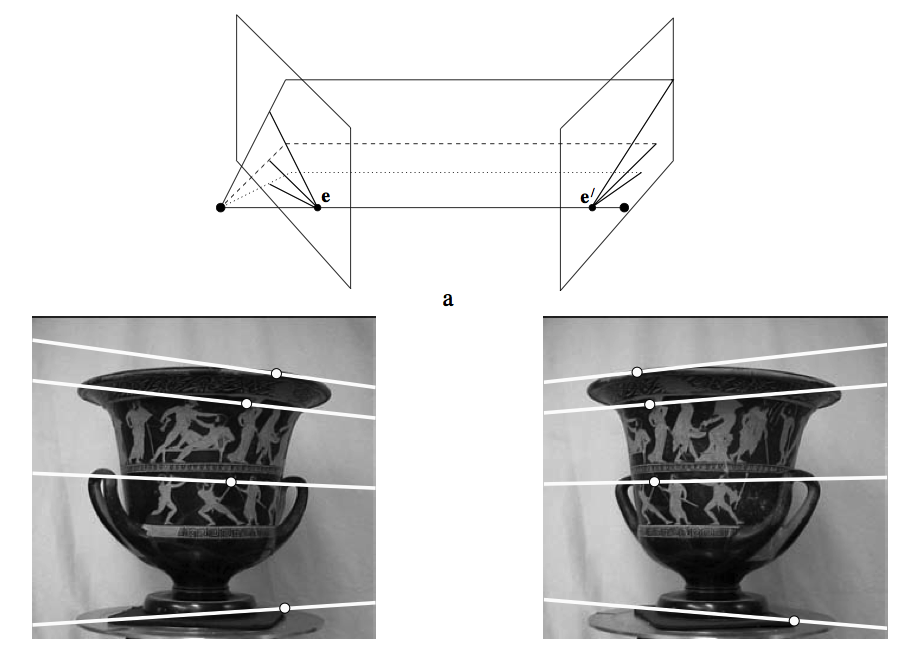
\includegraphics[width=0.8\textwidth]{EpipolarGeometry}
    \caption{Epipolar lines found in an image of a vase TODO reference}
    \label{fig:EpipolarGeometry}
\end{figure}
When enough inliers are found, points that do not satisfy the equation can be removed from further processing.
Once internal camera parameters K are known, the image points found can be calibrated and expressed in camera reference position system. Such calibrated points satisfy the following essential matrix E equation:
\begin{equation} \label{eq:essentialEquation}
{x}_{c}^{'T} * E * x_{c} = 0
\end{equation} 
which is very similar to fundamental equation \ref{eq:fundamntalEquation}. This results in:
\begin{equation} \label{eq:essentialFundamentalRelation}
E = K^{T} * F * K
\end{equation} 
with $K$ being the internal camera parameters. This equation \ref{eq:essentialFundamentalRelation} is important in terms of decomposition of F matrix to relative rotation and translation.
\subsection{Camera parameters estimations}
Internal camera parameters are expressed by the following matrix:
\begin{equation}
\begin{bmatrix}
\alpha _{x} &  & x_{0} \\ 
 & \alpha _{y} & y_{0}\\ 
 &  & 1
\end{bmatrix}
\end{equation}
where αx = fmx and αy = fmy represent the focal length of the camera expressed in pixel dimensions in the x and y direction respectively. 
Similarly, x ̃0 = (x0,y0) is the principal point of pixel dimensions. These parameters need to be calculated only once for each camera model. Cameras can be calibrated with special reference boards of the known dimensions and chracteristics.
For the proper 3D reconstruction it is essential to properly estimate external camera parameters, such as rotation (orientation angles of the camera) and global postition of the camera. It is often the case in 3D reconstruction that these parametrs are not known. However, it is showed in Chapter 9 of Multiple View Geometry in Computer Vision (\cite{HartleyMultipleView}), how essential matrix can be decomposed using Singular Value Decomposition \gls{svd} to relative camera positioning system of two projections:
\begin{equation}
 P1 = K * \begin{bmatrix}I\mid 0\end{bmatrix}
\end{equation}
the second one is equal to 
\begin{equation}
 P2 = K * \begin{bmatrix}RDiff\mid tDiff\end{bmatrix}
\end{equation}
Unfortunately, there are four possible solutions for such a decomposition and it is not always possible to identify the correct one.
\subsection{Points Triangulation}
Once internal and external (global or relative) camera parameters are calculated, the triangulation can be performed in order to acquire an up-to-affine reconstruction model (\ref{eq:3Dreconstruction}).
\begin{figure}[p]
    \centering
    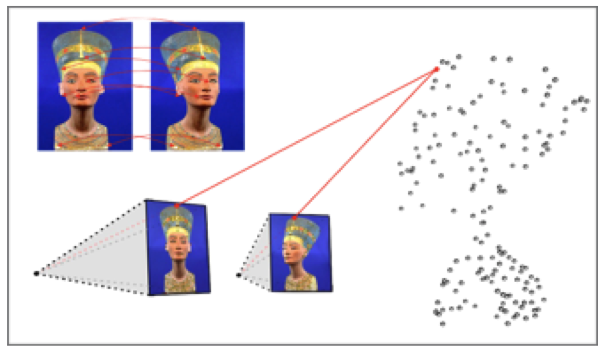
\includegraphics[width=0.8\textwidth]{3Dreconstruction}
    \caption{}
    \label{fig:3Dreconstruction}
\end{figure}
The only elemnt that cannot be determined in such a relative case is the scale. This process is described in detail in [TODO hartley chapter 10].
\section{Structure from Motion}
The term "Structure from Motion(SfM)" refers to the reconstruction performed from the consecutive sequences of a moving camera. It is a popular research topic and the two main approaches, namely the Pose Estimation and Homography Estimation, can be used for the [urposes of reconstructing a 3D model of an object.
\subsection{3D Pose Estimation}
Assuming that some of the 3D cloud points are already known, the matches between 2D features in a new image and 3D point cloud positions can be established. Such 3D-2D matches can be used to estimate the camera position. This allows for reconstructing new 3D points and merging them smoothly into a functional model. Unfortunately,  this process is also highly sensitive to the occurence of outliers, therefore adequate measeures have to be undertaken to reduce their influence. One of the main advanteges of this method is its speed. On the other hand, its effectiveness relies strongly on the exising 3D cloud quality. 
\subsection{Homography estimation}
A new image can be reconstructed with a previous one in a standard way in order to recive an up-to-scale 3D model. Afterwards, a newly acquired model can be merged into existing one using homography estimation between the coresponding 3D points. Such a strategy is slower than the previous one, but it is not influenced by the quality of the existing 3D model. Although it is highly sensitive to outliers as well, if used properly it can produce more new 3D points.
\subsection{Structure Adjustment}
Special refinement methods can be used to compensate for an error of mismatched points propagating through images. They include. among others, Bundle Adjustment\gls{ba} \url{http://en.wikipedia.org/wiki/Bundle_adjustment}. The algorithm, using the information concerning the corresponding matches between multiple sets of images, iteratively modifies either both the camera external paramaters and 3D points positions or one of them. The main disadvantage of the method is its execution time. It is too time-consuming to use it in real-time applications. The basic idea of BA is expresed in figure \ref{fig:BundleAdjustment}.
\begin{figure}[p]
    \centering
    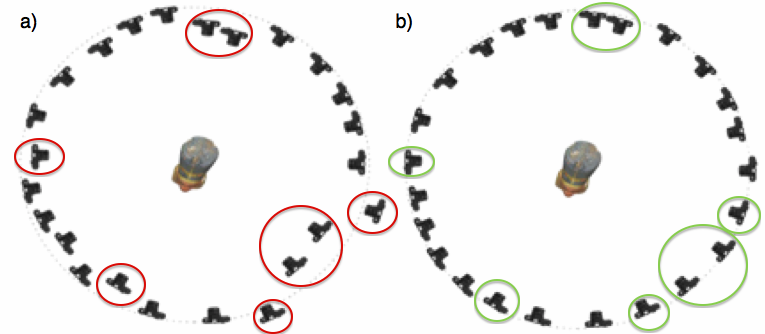
\includegraphics[width=0.8\textwidth]{BundleAdjustment}
    \caption{TODO reference}
    \label{fig:BundleAdjustment}
\end{figure}
\section{Mobile Sensors overview}
There are many sensors available in nowadays smartphones such as accelerometer, gyroscope, magnetomere, barometer, GPS etc. All of them have their advanteges and disadvanteges, but their errors, different in nature, can be compansated with each other to for exmaple accuretly compute camera rotation angles.
\subsection{Accelerometer}
An accelerometer is a device that measures acceleration along 3 axes of the device[reference]. Generally, accelerometers alows to measure total acceleration by sensing how much mass presses on its micro strings when a force is applied. An accelerometer, which lay on a flat surface perpendicular to the Earth's surface will indicate approximately 1G upwards. This gravitation vector can be used to caculate relative camera rotation, but it's hard to tell where in which direction gravity vector points, when device is moving in not linear manner. To obtain the gravity vector and track it during unexpected movement gyroscope sensor can be used.
\subsection{Gyroscope}
A gyroscope is a device for measuring or maintaining orientation, based on the principles of conservation of angular momentum [reference]. A standard gyroscope consists of a spinning wheel mounted on two gimbal rings, which allow it to rotate in all three axes. The spinning wheel will resist changes in orientation, due to an effect of the conservation of angular momentum. A conventional gyroscope measures orientation, in contrast to MEMS (Micro Electro-Mechanical System) types, which measure
angular rate, and are therefore called rate-gyros [reference]. MEMS gyroscopes contain vibrating elements to measure the Coriolis effect. In the end the angular velocity can be calculated in each axis. It is important to note that whereas the accelerometer and the magnetometer measure acceleration and angle relative to the Earth, gyroscope measures angular velocity
relative to the body.
\subsection{Magnetometer}
A magnetometer is an instrument used to measure the strength and/or direction of the magnetic field in the surrounding area of the instrument. It's main idea works the same as conventional compass. With some magentometers magnetic field can be me in 3 particular directions, relative to the spatial orientation of the device [reference]. Using magnetometers allows for relative position estimation in geomagnetic north position system. 
\subsection{Sensor Fusion}
Sensor fusion is the process of  combining sensory data derived from sensory data from disparate
sources such that the resulting information is in some sense better than would be possible
when these sources were used individually. The term better in this case can mean more
accurate, more complete, or more dependable, or refer to the result of an emerging view, such
as stereoscopic vision (calculation of depth information by combining two-dimensional
images from two cameras at slightly different viewpoints) [reference]. One of the possible strategies is Kalman-filterring(\ref{fig:Kalmann})
\begin{figure}[p]
    \centering
    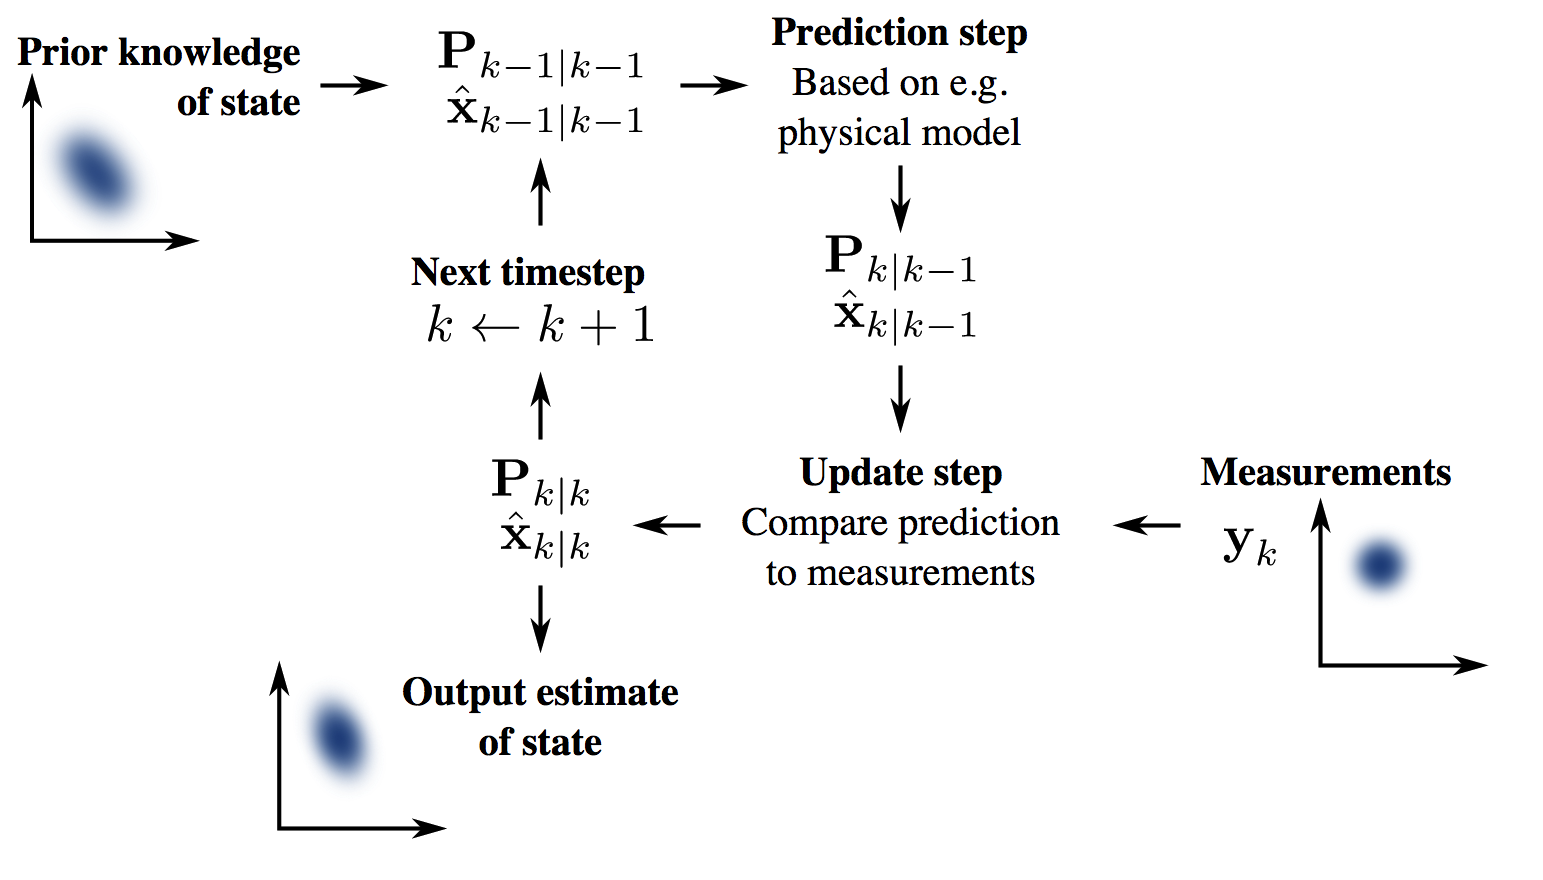
\includegraphics[width=0.8\textwidth]{Kalmann}
    \caption{}
    \label{fig:Kalmann}
\end{figure}
Available in Android API SesnorFusion sensor uses this approach, where the base of orientation measurements is calculation of gravity, when device was not moving and using gyroscope data (very accurate for a short period of time), when device starts to unexpectedly moving. Magnetometer data are fusined to allow for global earth coordinate system.


% ---------------------------------------------------------------------------
% ----------------------- end of thesis sub-document ------------------------
% ---------------------------------------------------------------------------
						% aims of the project
% this file is called up by thesis.tex
% content in this file will be fed into the main document

%: ----------------------- name of chapter  -------------------------
\chapter{Related Work} % top level followed by section, subsection
There are many approaches to the reconstruction problems, starting with the raw one-by-one pixel analysis for density matching, through high level abstraction of objects recognition and extraction and ending with the light and shadows-based reconstruction \cite{objectRecAndLoc}\cite{combinedMonoSlam}.
However this thesis does not focus on high-level abstraction reconstruction, but on refining relative poses estimation steps. As described in the theoretical part, in order to estimate the first two relative camera positions, an essential matrix must be decomposed. 
Since the basic epipolar geometry equation discovery, many scientist have introduced various ways to solve this linear problems, wchich differed primarily in terms of the accuracy and speed. One of the first was the 8-point algorithm \cite{8Point}, which can be used to compute a fundamental matrix. This can be done without any prior knowledge of the scene or camera external and internal parameters. Fundamental matrix has to be converted to essential matrix in order for the relative camera positions to be found and that is why it is necessary to calculate internal camera parameters. Next, the 5-point algorithm approaches were introduced \cite{Batra5point} \cite{Nister5point}. They used internal camera parameters for the proper essential matrix estimation. In his paper M. David Nister showed that the 5-point algorithm outperforms almost all similar algorithms in terms of accuracy and speed. Only the 8-point algorithm can be regarded as equally efficient. One of the state-of-art real-time and robust approaches is the iterative 5-point algorithm created by Vincent Lui and Tom Drummond\cite{iterative5point}.

Most of the algorithms are very sensitive to the occurence of outliers. One of the most common approaches to use to tackle this problem is RANSAC modelling\cite{RansacRefine}.

A research group from Technishe Universität Berlin made an interesting comparison and evaluation of the methods discovered by 2008 \cite{HellwichEvaluation}. It was discovered that estimation of camera rotation is much more stable than translation calculation. Furthermore, there are a lot of ambiguities regarding the choice of the correct solution of epipolar geometry equation. 

In certain situations, where external camera parameters as rotation and translation can be measured, more accurate algorithms were proposed.  In 2011 D. Scaramuzza from Zurich proposed a 1-point algorithm \cite{1point}, which shows how to describe and use a model of a camera mounted on a car to enhance 3D reconstruction. The 4-point algorithm introduced in 2013 using information of rotation angle in certain axis from additional sensor, as shown in paper \cite{4point}, can outperform even the 5-point algorithms. Lately the scientists have been creating more complex models to estimate relative stereometry, e.g. a team from Zurich proposed a way to enhance reconstruction with additional 6DOF sensor \cite{robustCameraImu}.

There are also non standard approaches like \cite{lineBasedPose}, where it is shown how to estimate the relative pose from three lines with two of the lines being parallel and orthogonal to the third one. Very accurate estimations can also be obtained for special camera model cases, when there is no rotation\cite{pureTransl}. All these references show that enhanced models often help to achieve more accurate or faster solutions to standard epipolar geometry problems.

Accuracy and speed constitute significant elements of the process of creating the systems capable of augmenting our reality. One of the first successful tracking and mapping reconstruction-based system was proposed by a research team from Oxford University \cite{ptam}. They showed how two simultaneously working threads can be used to both create a model of the environment being scanned and use this knowledge to apply graphical effects to objects presented on a video stream. Some of these concepts have already been applied to robotic vision. The authors showed efficiency of the proposed system for a robot walking in cluttered indoor workspaces\cite{monoSlam}. There were also approaches of porting reconstruction strategies to mobile devices\cite{simultanousRecLocMap} \cite{distributedAR} \cite{combinedMonoSlam} \cite{homographyMobile}.

The major conclusions to be drawn include the fact that rotation estimation is more stable than translation estimation and that the reconstruction accuracy is improved by a better described model of camera movement. Some of the researches drafted many scientific papers regarding rotation-improved solution space searching \cite{rotationSpaceSearch} \cite{Enqvist10stablestructure}. There are even some approaches involving the use of additional IMU accelerometer for the reconstruction process enhancement \cite{robustCameraImu}.


% ---------------------------------------------------------------------------
%: ----------------------- end of thesis sub-document ------------------------
% ---------------------------------------------------------------------------
			
% this file is called up by thesis.tex
% content in this file will be fed into the main document

%: ----------------------- name of chapter  -------------------------
\chapter{Concept} % top level followed by section, subsection
As indicated in a similar research it is very attractive to use additional data to enhance reconstruction and reduce ambiguity in finding correct solution for 3D reconstruction. Additional camera or model information help to implement faster, more stable and robust algorithms. This thesis will show how the prior knowledge of rotation or translation acquired via mobile sensor fusion can be used to enhance process of 3D reconstruction from a series of images. When it comes to relying on hand-held smartphones, the collected sensor data are very noisy. This thesis shows how even noisy information can be used in the reconstruction processes. Initially, only the camera rotation estimation was supposed to be used within the scope of this thesis. However, the first attempts to perform reconstruction proved it to be not sufficient and additional rotation error matrix estimations were developed.
It follows from the analysis of the theory and related works that both epipolar equations and pose estimation techniques can be improved by additional rotation and translation information data.  Author of this thesis proposes the use of an environment, where a user can decide what type of strategy to use.
\section{Requirements}
The proposed methodology needs an input in the form of a series of images with additional information about the position of the camera - the euclidan rotation and, optionally, translation. The use of smartphone is not necessary; any camera with sensor-fusioned accelerometer and gyroscope (magnotometer and the use thereof is optional, as discussed in [TODO], has both advantages and disadvantages), capable of performing the rotation and translation estimation, can be used.The internal camera parameters need to be calculated before the reconstruction process commences. Additional sensor data need not be fully accurate. Noisy external camera parameters can still be successfully used for enhancing the reconstruction process.
\section{Enhancing epipolar geometry equations with initial rotation matrix}
The initial pair reconstruction step is of utmost importance and needs to be accurate in order to let the other images calculate relative position based on the initially reconstructed 3D cloud points.
Analysis of the standard fundamental geometry equation and the relative camera based system ($P = \begin{bmatrix}I |0\end{bmatrix}, P' = \begin{bmatrix}R|t\end{bmatrix}$) results in the following:
\begin{equation} \label{eq:relativeFundamntal}
{x}_{'}^{T} * K^{-T} * \begin{bmatrix}T\end{bmatrix}_{x} * R * K^{-1} * x = 0
\end{equation}
It can also be noted that:
\begin{equation} \label{eq:skewTranslation}
\begin{bmatrix}T\end{bmatrix}_{x} = 
\begin{bmatrix*}[c]
 0 & -t_{z} & t_{y}\\
 t_{z} & 0 & -t_{x}\\
-t_{y} & t_{x} & 0 
\end{bmatrix*} 
where T = \begin{bmatrix}t_{x},t_{y},t_{z}\end{bmatrix}
\end{equation}
As already discussed, rotation can be distorted with noise. This can be written down as:
\begin{equation} \label{eq:Rerror}
R = R_{error} * R_{init} 
\end{equation}
where $R_{init}$ is initial rotation matrix constructed from the measured angles and $R_{error}$ is rotation error matrix.
Looking at this from a different point of view \ref{eq:Rerror} one can interpret it as the multiplication of the two rotation matrices: 
nne estimated, but close to local optimum initial rotation matrix and the second one responsible for correction of noise error. 
Instead of on the relative rotation matrix calculation, the primary idea of the algorithm proposed in this thesis is based on the entire rotation matrix calculation, which can be acquired from the essential matrix SVD decomposition, where only the rotation $R_{error}$ can be estimated. Eventually, \ref{eq:relativeFundamntal} can be rewritten as:
\begin{equation} \label{eq:relativeFundamntalEnhanced}
{x}_{'}^{T} * K^{-T} * \begin{bmatrix}T\end{bmatrix}_{x} * R_{error} * R_{init} * K^{-1} * x = 0
\end{equation}
Having:
\begin{equation} \label{eq:leftRelative}
\begin{array}{lcl}
h_{'}^{T} &=& {x}_{'}^{T} * K^{-T} \\
h &=& R_{init} * K^{-1} * x \\
G &=& \begin{bmatrix}T\end{bmatrix}_{x} * R_{error} \\
\end{array}
\end{equation}
With such notation one can notice that:
\begin{equation} \label{eq:alternativeEnhancedEquation}
{h}_{'}^{T} * G * h = 0
\end{equation}
which resembles the already known fundamental(\ref:{eq:fundamntalEquation}) and essential equations (\ref{eq:essentialEquation}). Naturally, $h_{'}$ and h both are expressed in homogenous coordinates. Tt follows from the analysis that G has 6DOF: 3 due to an unknown translation and another 3 due to an unknown correction angles (created by rotation error matrx decomposition). Theoretically, such matrix can be resolved for instance by both 5 and 8-point algorithms. Therefore the standard fundamental and essential equation solvers can be used in order to retrieve both $\begin{bmatrix}T\end{bmatrix}_{x}$ and $R_{error}$.
The finally estimated $R_{error}$ and calculated $R_{init}$ has to be multiplied in order for the new rotation estimation of R (\ref{eq:Rerror}) to be retrieved.
Pursuant to Appendix 6 "Multiple View Geometry in Computer Vision"(A6.9.1 \cite{HartleyMultipleView}), the use of Rodigues parametrization for small angles (and noise in initial rotation matrices estimations can be expresed by small angles) the rotation matrix, and thus $R_{error}$, equals approximately to:
\begin{equation} \label{eq:rodiguesError}
R_{error} \cong 
\begin{bmatrix*}[c]
    1   &  -w_{z}&  w_{y}\\ 
 w_{z}  &    1   & -w_{x}\\
-w_{y}  &  w_{x} &   1
\end{bmatrix*}
\end{equation} 
Such a criterion with a special matrix design can be used when decomposing G to resolve some ambiguity in choosing the proper solution. The standard four solution ambiguity with two possible rotations and translations can be reduced to two possible translation calculations. The concept described constitutes a basis of the implemented, enhanced 8-point and 5-point algorithms.

\subsection{Alternative 3-point algorithm for finding the translation}
Following the \ref{eq:alternativeEnhancedEquation} it can be stated that:
\begin{equation} \label{eq:alternative3point}
{x}_{'}^{T} * K^{-T} * \begin{bmatrix*}[c]
 0 & -t_{z} & t_{y}\\
 t_{z} & 0 & -t_{x}\\
-t_{y} & t_{x} & 0 
\end{bmatrix*} * R * K^{-1} * x = 0
\end{equation}
Having:
\begin{equation} \label{eq:leftRelative}
\begin{array}{lcl}
h_{'}^{T} &=& {x}_{'}^{T} * K^{-T} \\
h &=& K^{-1} * x \\
\end{array}
\end{equation}
and 
\begin{equation} \label{eq:alternative3point}
\begin{bmatrix*}[c]
h_{'1} & h_{'2} & h_{'3}
\end{bmatrix*}
* \begin{bmatrix*}[c]
 0 & -t_{z} & t_{y}\\
 t_{z} & 0 & -t_{x}\\
-t_{y} & t_{x} & 0 
\end{bmatrix*} 
* \begin{bmatrix*}[c]
h_{1} \\
h_{2} \\
h_{3}
\end{bmatrix*}
= 0
\end{equation}
and multiplying it one receives the following:
\begin{equation} \label{eq:alternative3point}
h_{1}*h_{'2}*t_{z} - h_{1}*h_{'3}*t_{y} - h_{2}*h_{'1}*t_{z} + h_{2}*h_{'3}*t_{x} + h_{3}*h_{'1}*t_{y} - h_{3}*h_{'2}*t_{x}
= 0
\end{equation}
what can be grouped:
\begin{equation}
t_{x} * (h_{2}*h_{'3} - h_{3}*h_{'2}) + t_{y} * (h_{3}*h_{'1} - h_{1}*h_{'3}) + t_{z} * (h_{1}*h_{'2} - h_{2}*h_{'1}) = 0
\end{equation}
and rewritten as:
\begin{equation} \label{eq:translation3point}
\begin{bmatrix*}[c]
t_{x} &
t_{y} &
t_{z}
\end{bmatrix*} * \begin{bmatrix*}[c]
(h_{2}*h_{'3} - h_{3}*h_{'2}) \\ 
(h_{3}*h_{'1} - h_{1}*h_{'3}) \\
(h_{1}*h_{'2} - h_{2}*h_{'1}) 
\end{bmatrix*} 
= 0
\end{equation}
then solved for instance with SVD with only three points. This is a truly fast way of estimating translation for the reconstructed images. However, in such situation the overall accuracy strictly depends on the precise measuerments of camera orientation.
\section{Pose estimation}
One of the main goal was to develop a more accurate and faster version of the reconstruction algorithm. That is why the relative pose estimation techniques were used to enrich models with additional points. In general, this approach produces less outliers than the homography merging techniques. This also allows to maintain the scale of the reconstructed images. For any point of the image, which has a corresponding 3D point the following condition is met:
\begin{equation} \label{eq:projectionEquation}
 x = P * X
\end{equation}
where x is image point expressed in homogenous coordinates (x , y , 1) and X homogenous 3D point (X , Y , Z , 1). 
The projection matrix of the camera design is as follows: 
\begin{equation} \label{eq:projectionEquation}
 P = K * \begin{bmatrix}R\mid t\end{bmatrix}
\end{equation}
\subsection{Rotation enhancements}
Applying the similar approach to initial pair reconstruction enhancements, it can be noted that:
\begin{equation} \label{eq:projectionRotError1}
\begin{array}{rcl}
 x & = & K * \begin{bmatrix}Rinit + dR\mid t\end{bmatrix} * X \\
 x & = & K * \begin{bmatrix}Rinit\mid 0\end{bmatrix} * X + K * \begin{bmatrix}dR\mid t\end{bmatrix} * X \\
 x - K * \begin{bmatrix}Rinit\mid 0\end{bmatrix} & = & K * \begin{bmatrix}dR\mid t\end{bmatrix} * X
\end{array}
\end{equation}
Substituting $x_{m} = x - K * \begin{bmatrix}Rinit\mid 0\end{bmatrix}$ the following is received: 
\begin{equation} \label{eq:projectionRotError2}
x_{m} = K * \begin{bmatrix}dR\mid t\end{bmatrix} * X
\end{equation}
This can be solved using a standard PNP calculating algorithms. Rotation can be used as an initial solution for the pose estimation in order to focus solely on the rotation error and translation estimation.
\subsection{Rotation \& translation enhancements}
Similar to \ref{eq:projectionRotError1}:
\begin{equation} \label{eq:projectionRotError3}
\begin{array}{rcl}
 x & = & K * \begin{bmatrix}Rinit + dR\mid Tinit + dt\end{bmatrix} * X \\
 x & = & K * \begin{bmatrix}Rinit\mid Tinit\end{bmatrix} * X + K * \begin{bmatrix}dR\mid dt\end{bmatrix} * X \\
 x - K * \begin{bmatrix}Rinit\mid Tinit\end{bmatrix} & = & K * \begin{bmatrix}dR\mid dt\end{bmatrix} * X
\end{array}
\end{equation}
end in the end by substituting $x_{n} = x - K * \begin{bmatrix}Rinit\mid Tinit\end{bmatrix}$ the following is receivedt: 
\begin{equation} \label{eq:projectionRotError4}
x_{n} = K * \begin{bmatrix}dR\mid dt\end{bmatrix} * X
\end{equation}
This can also be solved using a standard PNP[TODO reference] calculation algorithm. Rotation and translation can be used as an initial solution for the pose estimation in order to focus solely on the rotation error and translation error estimation.
\section{Known rotations \& translations}
Where accurate rotations and translations of cameras are known, no aditional pose calculations are needed. Such a situation is interesting, since everything needed for corresponding points triangulation is already known. However, mobile sensor data  measurements are very noisy. In that case Bundle Adjustment can be used in order to refine the measured calculated camera positions and the final 3D cloud reconstruction.
\section{Reconstruction process strategy}
Finally, all methods described herein can be combined in different reconstruction strategies. For the initialization of 3D cloud point the following strategies can be used: 
%TODO zrobić lepszy styl
\begin{enumerate} 
\item \textbf{Known rotations and translations}, which theoritcally allows for an up-to-metrical reconstruction
\item \textbf{Known rotations}, where translation is estimated with an alternative 3-point algorithm
\item \textbf{Noisy rotations}, where enhanced 8-point fundamental or 5-point essential algorithms are used in order to calculate rotation error and relative translation 
\item \textbf{Unknown external camera parameters}, where standard 8-point fundamental or 5-point essential algorithms are used in order to calculate rotation and relative translation
\end{enumerate}
For the pose estimation the following methodologies can be used:
\begin{enumerate}
\item \textbf{Known rotations and translations}, where no additional calculations are required and an up-to-metrical model can be acquired
\item \textbf{Initial rotation}, where relative translation needs to be calculated
\item \textbf{Noisy rotation and translation}, where both rotation and translation errors need to be calculated
\item \textbf{Unknown external camera parameters}, where standard pose estimation has to be used
\end{enumerate}

% ---------------------------------------------------------------------------
%: ----------------------- end of thesis sub-document ------------------------
% ---------------------------------------------------------------------------


% this file is called up by thesis.tex
% content in this file will be fed into the main document

%: ----------------------- name of chapter  -------------------------
\chapter{Implementation} % top level followed by section, subsection


%: ----------------------- contents from here ------------------------

\section{Environment}
\section{Project Structure}
\subsection{Android application}
\subsection{OSX CMake base project}
\section{Important Implementation Aspects}
\subsection{Custom Sensor Data File format}
\section{Graphical User Interface}
\section{Documentation}





% ---------------------------------------------------------------------------
%: ----------------------- end of thesis sub-document ------------------------
% ---------------------------------------------------------------------------


% this file is called up by thesis.tex
% content in this file will be fed into the main document

% change according to folder and file names
\ifpdf
    \graphicspath{{figures/}{figures/comparisons}}
\else
    \graphicspath{{figures/}{figures/comparisons}}
\fi


\chapter{Evaluation} % top level followed by section, subsection
All implemented algorithms were tested in terms of speed, accuracy and effectiveness. As regards the speed test, it included the measurement of the reconstruction execution time. In the accuracy testing Sampson Error measurement was used (this variable measures the distance between all points and their corresponding epipolar lines in an image). Effectiveness was tested using visual comparison of reconstructed 3D cloud points.
% ----------------------- contents from here ------------------------
\section{Acquiring datasets}
For the purpose of analysis the following datasets were captured with implemented "Sensor Enhanced Images Camera" and Nexsus 5 camera:
\begin{enumerate}
\item Warsaw University of technology main building(4 images 1024x768pixels)
\item Advertisment Pole ??? 
\item Warsaw Buisness School Gate and Entrance ??
\item Warsaw Shopping Center Back???
\item Warsaw Shopping Center Front???
\end{enumerate}
Since most of the algorithms proposed in the (TODOreference to Concept) Concept section require internal camera parametrs to be known, the camera used in the course of conducting this study was calibrated and its parameters were stored in $"out_camera_data.yml"$ file. All of these datasets can be found in attached CD or Github repository.
\section{Test Environment}
All tests were perfomed on MacBook Air with 1.7GHz dual-core Intel Core i7 processor and 8GB 1600MHz DDR3 RAM using "Enhanced 3D Reconstructer" implemented as described in Implementation section.  Numerical tests which allowed for measuring total errors and execution time were run on "Warsaw University of Technology" dataset. Initial pair reconstruction ability of each method proposed was measured as well as various reconstruction strategies.  Finally, for each dataset the most effective methods were used to reconstruct sparse models. 
\section{Testing initial pair reconstrucion methods} \label{sec:Testin2Views}
The key question to be answered at this point was whether the proposed sensor enhancement gave better results than standard algorithms.
The following methods were tested: TODO methods should be already described in Concept and implementation
\begin{enumerate}
\item \textbf{Standard 8-point} - based on [] Fundamental matrix decomposition, implemented in OpenCV
\item \textbf{Enhanced 8-point} - proposed camera rotation enhanced version of above 8-point algorithm
\item \textbf{Alternative 3-point} - proposed 3-point algorithm to translation estimation.
\item \textbf{Known rotations and translations} - calculation from known cameras rotations and translations
\item \textbf{Standard essential 5-point} - based on [] Essential matrix decomposition, implemented in []
\item \textbf{Enhanced essential 5-point} - similar to 2. improvements rotation enhanced version of above 5-point algorithm
\end{enumerate}
\subsection{Accuracy - Epipolar lines correspondence}
In the case of initial pair images one of the most imporant factors include the epipolar constraint. Using a properly estimated fundamental matrix drawing corresponding epipolar lines in both images is possible. Furthermore, points lying on two matching epipolars lines in different images can be easily matched. In other words, epipolar lines cross exactly the same points in both images. The more accurate they are the more corresponding pairs can be found, e.g. for th epurposes of performing dense reconstruction. Sampson Error is one of metrics that can be used in order to estimate the accuracy of epipolars lines; the smaller the error's value the more accurate the lines. 
\begin{figure}[b!]
  \begin{center}
    \begin{tikzpicture}
      \begin{axis}[
          width=\linewidth, % Scale the plot to \linewidth
          grid=major, % Display a grid
          grid style={dashed,gray!30}, % Set the style
          xtick = {100,500,1000,5000},
          xlabel=Sift features number, % Set the labels
          xmode=log,
          log ticks with fixed point,
          ymode=log,
          log ticks with fixed point,
          ylabel=Total Sampson Error(pixels),
          legend style={at={(0.5,-0.05)},anchor=north,cells={anchor=west}}, % Put the legend below the plot
        ]
        \addplot[mark=*,blue] table[x=Number of Sift features,y=8-point OpenCV,col sep=comma] {SampsonTotal.csv}; 
        \addplot[mark=*,red] table[x=Number of Sift features,y=8-point enhanced,col sep=comma] {SampsonTotal.csv};
        \addplot[mark=*,orange] table[x=Number of Sift features,y=Alternative 3-point,col sep=comma] {SampsonTotal.csv}; 
        \addplot[mark=*,pink] table[x=Number of Sift features,y=Known rot and trans,col sep=comma] {SampsonTotal.csv};
        \addplot[mark=*,green] table[x=Number of Sift features,y=Essential 5-point,col sep=comma] {SampsonTotal.csv};
        \addplot[mark=*,yellow] table[x=Number of Sift features,y=5-point enhanced,col sep=comma] {SampsonTotal.csv};
        \legend{Standard 8-point,Enhanced 8-point,Alternative 3-point,Known rotations and translations,Standard essential 5-point,Enhanced essential 5-point}
      \end{axis}
    \end{tikzpicture}
    \caption{Chart showing the sum of Sampson Errors in a picture(1024x768pixels) per various initial SIFT features sets sizes}
    \label{plot:TotalSampsonError}
  \end{center}
\end{figure}
Its primary function is to measure the sum of distance between all points and their corresponding epipolar lines. However, each of proposed methods has different outliers removal capabilities, therefore in order to compare their efficiency the average of Samson Error per a corresponding pair was calculated.
The following chart \ref{plot:TotalSampsonError} shows the total Sampson Errors for different sets of initial SIFT features. The major observation made based on these results is that most of the algorithms remove outliers properly. As could have been expected the only one that is not efficient in this regard is the method involving drawing epipolar lines from heuristically estimated movement and noisy rotation, which produces significantly larger error than the other algorithms.
\begin{figure}[hb!]
  \begin{center}
    \begin{tikzpicture}
      \begin{axis}[
          width=\linewidth, % Scale the plot to \linewidth
          grid=major, % Display a grid
          grid style={dashed,gray!30}, % Set the style
          xtick = {100,500,1000,5000},
          xlabel=Sift features number, % Set the labels
          xmode=log,
          log ticks with fixed point,
          ymode=log,
          log ticks with fixed point,
          ylabel=Total Sampson Error per point(pixels),
          legend style={at={(0.5,-0.05)},anchor=north,cells={anchor=west}}, % Put the legend below the plot
        ]
        \addplot[mark=*,blue] table[x=Number of Sift features,y=8-point OpenCV,col sep=comma] {SampsonPerPoint.csv}; 
        \addplot[mark=*,red] table[x=Number of Sift features,y=8-point enhanced,col sep=comma] {SampsonPerPoint.csv};
        \addplot[mark=*,orange] table[x=Number of Sift features,y=Alternative 3-point,col sep=comma] {SampsonPerPoint.csv}; 
        \addplot[mark=*,pink] table[x=Number of Sift features,y=Known rot and trans,col sep=comma] {SampsonPerPoint.csv};
        \addplot[mark=*,green] table[x=Number of Sift features,y=Essential 5-point,col sep=comma] {SampsonPerPoint.csv};
        \addplot[mark=*,yellow] table[x=Number of Sift features,y=5-point enhanced,col sep=comma] {SampsonPerPoint.csv};
        \legend{Standard 8-point,Enhanced 8-point,Alternative 3-point,Known rotations and translations,Standard essential 5-point,Enhanced essential 5-point}
      \end{axis}
    \end{tikzpicture}
    \caption{Chart showing per point Sampson Error in a picture(1024x768pixels) per various initial SIFT features sets sizes}
    \label{plot:SampsonErrorPerPoint}
  \end{center}
\end{figure}
Analysing the Per Pair Sampson Error results \ref{plot:SampsonErrorPerPoint} it can be noted that the proposed sensor enhanced methods did not improve either the 8-point or 5-point algorithms, but the 3-point algorithm developed for the purposes of this thesis proved to be much faster than the 8-point algorithm and also quite accurate. To present the discussed errors, estimated epipolar lines for 300 initial SIFT features set were drawn on the figures \ref{fig:SummaryEpiLines1300} - \ref{fig:SummaryEpiLines2300}.
\begin{figure}[b!]
    \centering
    \includegraphics[width=0.8\textwidth]{summary1Sift300}
    \caption{The results of drawing estimated epipolar lines on Warsaw Univeristy Dataset with 300 SIFT points. 1) Standard Fundamental 8-point algorithm (upper pair), 2) Rotation Enhanced Fundamental 8-point algorithm (middle pair), 3) Alternative 3-point algorithm (bottom pair) }
    \label{fig:SummaryEpiLines1300}
\end{figure}
\begin{figure}[ht!]
    \centering
    \includegraphics[width=0.8\textwidth]{summary2Sift300}
    \caption{The results of drawing estimated epipolar lines on Warsaw Univeristy Dataset with 300 SIFT points. 1) Fundamental matrix created from rotation and translation (upper pair), 2) Standard Essential matrix 5-point algorithm (middle pair), 3) Rotation Enhanced Essential 5-point algorithm (bottom pair) }
    \label{fig:SummaryEpiLines2300}
\end{figure}
It can be seen that both standard 8-point algorithm and the proposed rotation enhanced version return very good results in terms of epipolar lines accuracy. The alternative 3-point algorithm gives slightly worse results due to uncompansated mobile sensors noise. In this particular dataset the essential 5-point method was inefficient in producing proper essential matrix estimation, contrary to the proposed sensor enhanced 5-point algorithm, which found satisfactory correspondency in epipolar lines. \newline
To verify whether the epipolar lines calculation is influenced by the number of SIFT features, the same process was applied to 1000 SIFT features set(\ref{fig:SummaryEpiLines11000} - \ref{fig:SummaryEpiLines21000}). 
\begin{figure}[b!]
    \centering
    \includegraphics[width=0.8\textwidth]{summary1Sift1000}
    \caption{Results of drawing estimated epipolar lines on Warsaw Univeristy Dataset with 1000 SIFT points. 1) Standard Fundamental 8-point algorithm (upper pair), 2) Rotation Enhanced Fundamental 8-point algorithm (middle pair), 3) Alternative 3-point algorithm (bottom pair) }
    \label{fig:SummaryEpiLines11000}
\end{figure}
\begin{figure}[ht!]
    \centering
    \includegraphics[width=0.8\textwidth]{summary2Sift1000}
    \caption{Results of drawing estimated epipolar lines on Warsaw Univeristy Dataset with 1000 SIFT points. 1) Fundamental matrix created from rotation and translation (upper pair), 2) Standard Essential matrix 5-point algorithm (middle pair), 3)Rotation Enhanced Essential 5-point algorithm (bottom pair) }
    \label{fig:SummaryEpiLines21000}
\end{figure}
In general, the proposed enhanced algorithms are not better than standard versions in terms of accuracy of epipolar lines estimation. Mostly because during calculation some of the noise in sensor data is propagated on Epipolar geometry estiamion. However enhanced versions are always close to optimal solutions. Standard versions for instance can fail sometimes in terms of Fundamental matrix estimation.
\clearpage

\subsection{Time comparison}
On chart \ref{plot:ExecutionTime} avaraged  execution time for 100 estimation attempts was presented.
\begin{figure}[hb!]
  \begin{center}
    \begin{tikzpicture}
      \begin{axis}[
          width=\linewidth, % Scale the plot to \linewidth
          grid=major, % Display a grid
          grid style={dashed,gray!30}, % Set the style
          xtick = {100,500,1000,5000},
          xlabel=Sift features number, % Set the labels
          xmode=log,
          log ticks with fixed point,
          ymode=log,
          ylabel=Execution time(ms),
          legend style={at={(0.5,-0.05)},anchor=north,cells={anchor=west}}, % Put the legend below the plot
        ]
        \addplot[mark=*,blue] table[x=Number of Sift features,y=8-point OpenCV,col sep=comma] {ExecutionTime.csv}; 
        \addplot[mark=*,red] table[x=Number of Sift features,y=8-point enhanced,col sep=comma] {ExecutionTime.csv};
        \addplot[mark=*,orange] table[x=Number of Sift features,y=Alternative 3-point,col sep=comma] {ExecutionTime.csv}; 
        \addplot[mark=*,pink] table[x=Number of Sift features,y=Known rot and trans,col sep=comma] {ExecutionTime.csv};
        \addplot[mark=*,green] table[x=Number of Sift features,y=Essential 5-point,col sep=comma] {ExecutionTime.csv};
        \addplot[mark=*,yellow] table[x=Number of Sift features,y=5-point enhanced,col sep=comma] {ExecutionTime.csv};
        \legend{Standard 8-point algorithm,Enhanced 8-point algorithm,Alternative 3-point algorithm,Known rotations and translations,Standard essential 5-point algorithm,Enhanced essential 5-point algorithm}
      \end{axis}
    \end{tikzpicture}
    \caption{Execution time of proposed algorithms(1024x768pixels) in comparison to initial SIFT feature set}
    \label{plot:ExecutionTime}
  \end{center}
\end{figure}
Execution time of 8-point versions are very similar, which is understandable, because they implementation is pretty much the same and they differ only characteristic of analysed dataset. It can be seen that execution time of 5-point epipolar estimations versions differ much. In this situation either finding optimal solution with initial rotation is much harder or implementation of these methods are very different in terms of memory allocation. Execution time of 3-points algorithm is few times faster than 8-point algorithms. Estimation using only known rotations and translations has few times smaller order execution time than standard algorithms, but as we know from previous section gives uncorreleted epipolar lines.

\section{Testing reconstruction strategies}
As was shown in \ref{sec:Testin2Views} not every initial reconstruction methods gives good results. Only the most effective techniques were used to prepare few completely different strategies:
\begin{enumerate}
\item \textnormal{Standard 8-point + OpenCV Pose Estimation} 
\item \textnormal{Enhanced 8-point + OpenCV Pose Estimation} 
\item \textnormal{Enhanced 8-point + Initial Rotation and Translation OpenCV Pose Estimation} 
\item \textnormal{Alternative 3-point + OpenCV Pose Estimation}
\item \textnormal{Alternative 3-point + Initial Rotation and Translation OpenCV Pose Estimation}
%\item \textnormal{Known rotations and translations} 
\end{enumerate}
First method gives us basic reference to standard 3D reconstruction strategy. Second one was choosen, because extremly consistence in 3D reconstraction. It has never failed to produce solution close to optimal. Thrid was prepared in order to check, how enhanced Pose Estimation influence final reconstruction. Forth and fifth strategies were used to see, if models can be produced faster without much impact on final accuracy. Finally sixth one was proposed in order to check, wheter whole reconstruction process can be performed with only sensor data.

\subsection{Accuracy}
Accuracy of 3D reconstraction was measured using Bundle Adjustment algorithm from SBA library[ref]. It allows to calculate error based on projective constratin both before and after Bundle Adjustment.
Performed with different strategis tests for "Warsaw Univeristy" dataset were plotted on \ref{plot:BAError}. Big differences in initial error can be explained different number of reconstructed points after initial phase and inconsistent unknown scale of finally reconstracted models. Enhanced initial pair reconstruction and pose estimation methods have bigger impact on Bundle Adjustment error reduction.
\begin{figure}[ht!]
  \begin{center}
    \begin{tikzpicture}
      \begin{axis}[
          width=\linewidth, % Scale the plot to \linewidth
          grid=major, % Display a grid
          grid style={dashed,gray!30}, % Set the style
          xtick = {1,2,3,4,5},
          xticklabels = {Std8 -point+NormalPose,Enhanced8-point+NormalPose,Enhanced8-point+EnhancedPose, Alternative3-point+NormalPose,Alternative3-point+EnhancedPose},          
          xlabel=Reconstruction strategy, % Set the labels
          log ticks with fixed point,
          ymode=log,
          ylabel=Reconstruction error(in model units),
          x tick label style={rotate=90,anchor=east},
          legend style={at={(0.5,1.05)},anchor=south,cells={anchor=west}}, % Put the legend below the plot
        ]
        \addplot[mark=*,blue] table[x=ReconMethods,y=Error before BA,col sep=comma] {BAerror2.csv}; 
        \addplot[mark=*,red] table[x=ReconMethods,y=Error after BA,col sep=comma] {BAerror2.csv};
        \legend{Reconstruction Error before Bundle Adjustment,Reconstruction Error after Bundle Adjustment}
      \end{axis}
    \end{tikzpicture}
    \caption{Influence of Bundle adjustment on models produced with different reconstruction strategies }
    \label{plot:BAError}
  \end{center}
\end{figure}
\clearpage
In general, Bundle Adjustmet process allows to rearrange and modify 3D points positions and also change external paramaters of estimated cameras. However, in case of enhanced algoritms estimated camera positions are already very close to their optimal estimations.  Such situation allows Bundle Adjustment method to focus mainly on 3D points modifications. It can be seen that enhanced Pose Estimation in comparison to standard Pose Estimation results in further reduction of BA error. 

\subsection{Execution time}
In chart \ref{plot:ReconstructionWithoutBA} reconsturction execution time without Bundle Adjustment was presented. Comparing execution time of reconstruction using known rotations and translations from \ref{plot:ExecutionTime} one can see that most of the reconstruction time is used for SIFT correspondences matching. Proper correspondeces matching is bottle-neck in all implemented reconstruction strategies. Reconstruction time with Bundle Adjustment turned on was shown in chart\ref{plot:ReconstructionWithBA}). It turns out that Bundle Adjustment works much faster for strategies that used enhanced initial pair reconstructions and enhanced pose Estimation. As explained earlier such enhanced reconstructions are better organised than standard ones. This results in faster convergence of BA. Sample difference between reconstructed cloud points before and after BA can be seen in \ref{fig:BundleAdjustmentComparison}.
\begin{figure}[b!]
    \centering
    \includegraphics[width=\textwidth]{bundleAdjustmentComparison}
    \caption{3D point clouds before Bundle Adjustment(upper pair) and after(bottom pair) reconstructed using enhanced 8-point initial pair algorithm and enhanced Pose Estimation. Warsaw University of Technology dataset for 1000 SIFT corresponding features(left - front, right - from side)}
    \label{fig:BundleAdjustmentComparison}
\end{figure}
\begin{figure}[h!]
  \begin{center}
    \begin{tikzpicture}
      \begin{axis}[
          width=\linewidth, % Scale the plot to \linewidth
          grid=major, % Display a grid
          grid style={dashed,gray!30}, % Set the style
          xtick = {100,500,1000,5000},
          xlabel=SIFT features number, % Set the labels
          xmode=log,
          log ticks with fixed point,
          ymode=normal,
          ylabel=Execution time(ms),
          legend style={at={(0.5,-0.05)},anchor=north,cells={anchor=west}}, % Put the legend below the plot
        ]
        \addplot[mark=*,blue] table[x=Number of Sift features,y=8-pointInit+NormalPoseEstim,col sep=comma] {ReconstructTotal.csv}; 
        \addplot[mark=*,red] table[x=Number of Sift features,y=Enhanced8-point+NormalPoseEstim,col sep=comma] {ReconstructTotal.csv};
        \addplot[mark=*,orange] table[x=Number of Sift features,y=Enhanced8-point+EnhancedPoseEstim,col sep=comma] {ReconstructTotal.csv}; 
        \addplot[mark=*,pink] table[x=Number of Sift features,y=Alternative3-point+NormalPoseEstim,col sep=comma] {ReconstructTotal.csv};
        \addplot[mark=*,green] table[x=Number of Sift features,y=Alternative3-point+EnhancedPoseEstim,col sep=comma] {ReconstructTotal.csv};
%        \addplot[mark=*,yellow] table[x=Number of Sift features,y=Known Rotations and Translations,col sep=comma] {ReconstructTotal.csv};
        \legend{Standard 8-point initialization + Normal OpenCV Pose Estimation,Enhanced 8-point initialization + normal Pose Estimation,Enhanced 8-point initiazliation + enhanced Pose Estimation, Alternative 3-point initiazliation + normal Pose Estimation, Alternative 3-point initialization + enhanced Pose Estimation}
      \end{axis}
    \end{tikzpicture}
    \caption{Total reconstruction execution time (4 images with resolution 1024x768pixels) in comparison to Sift feature number}
    \label{plot:ReconstructionWithoutBA}
  \end{center}
\end{figure}

\begin{figure}[h!]
  \begin{center}
    \begin{tikzpicture}
      \begin{axis}[
          width=\linewidth, % Scale the plot to \linewidth
          grid=major, % Display a grid
          grid style={dashed,gray!30}, % Set the style
          xtick = {100,500,1000,5000},
          xlabel=SIFT features number, % Set the labels
          xmode=log,
          log ticks with fixed point,
          ymode=normal,
          ylabel=Execution time(ms),
          scaled ticks = false,
          xticklabel style={/pgf/number format/.cd,fixed,precision=5},
          legend style={at={(0.5,-0.05)},anchor=north,cells={anchor=west}}, % Put the legend below the plot
        ]
        \addplot[mark=*,blue] table[x=Number of Sift features,y=8-pointInit+NormalPoseEstim,col sep=comma] {ReconstructBA.csv}; 
        \addplot[mark=*,red] table[x=Number of Sift features,y=Enhanced8-point+NormalPoseEstim,col sep=comma] {ReconstructBA.csv};
        \addplot[mark=*,orange] table[x=Number of Sift features,y=Enhanced8-point+EnhancedPoseEstim,col sep=comma] {ReconstructBA.csv}; 
        \addplot[mark=*,pink] table[x=Number of Sift features,y=Alternative3-point+NormalPoseEstim,col sep=comma] {ReconstructBA.csv};
        \addplot[mark=*,green] table[x=Number of Sift features,y=Alternative3-point+EnhancedPoseEstim,col sep=comma] {ReconstructBA.csv};
%        \addplot[mark=*,yellow] table[x=Number of Sift features,y=Known Rotations and Translations,col sep=comma] {ReconstructTotal.csv};
        \legend{Standard 8-point initialization + normal OpenCV Pose Estimation,Enhanced 8-point initialization + normal Pose Estimation,Enhanced 8-point initiazliation + enhanced Pose Estim, Alternative 3-point initiazliation + normal Pose Estimation, Alternative 3-point initialization + enhanced Pose Estimation}
      \end{axis}
    \end{tikzpicture}
    \caption{Total execution time of reconstruction with Bundle Adjustment turned on(4 images with resolution 1024x768pixels) in comparison to initial SIFT feature set}
    \label{plot:ReconstructionWithBA}
  \end{center}
\end{figure}
\clearpage

\section{Effectivness}
However numerical measuerments do not always results in proper 3D model reconstructions, so some of the intresting 3D reconstraction situations are presented on next 4 pages. In \ref{fig:uni4000Comparison} different Initialization Pair methods were used to reconstruction models for 4000 SIFT features. It can be seen that standard and enhaced methods gave quite good results, which only differ in scale. 3-point algorithm produces quite good models, but slightly distorted due to noise in used rotations. Model reconstructed from known rotations and translations are very distorted, but stil readable. It could be used, when very fast reconstruction is needed. Essential Matrix estimation methods unfortunately failed in terms of relative pose estimation.
\newline
However situation changes a little bit for 400 points. Every algorithm managed to find solution reallt close to optimum. In some cases "Traingulation Test" used in Standard 8-point approach fails and produces unrecognizable model(\ref{fig:FailCaseFundamental}).
\newline
When it comes to Pose Estimations enhancments one can see in \ref{fig:PoseEstimationMethodComparison} that generally initial  rotation and translation help to find better solution, which mainly manifests in less outliers number.
\newline
In figure \ref{fig:UniNone4000} it can be seen, how many outliers using only noisy rotations and translations produces.
\newline
More reconstructed models can be found in [TODO Materials]
\begin{figure}[p]
    \centering
    \includegraphics[width=0.9\textwidth]{uni4000Comparison}
    \caption{Reconstructed models for proposed Initial reconstruction methods and 4000 SIFT Features. From upper left to bottom right following: 1) Standard 8-point, 2) Enhanced 8-point, 3) Alternative 3-point, 4) Known rotations and translations, 5) Standard 5-point, 6) Enhanced 5-point}
    \label{fig:uni4000Comparison}
\end{figure}
\begin{figure}[t!]
    \centering
    \includegraphics[width=0.9\textwidth]{uni400Comparison}
    \caption{Reconstructed models for proposed Initial reconstruction methods and 400 SIFT Features. From upper left to bottom right following: 1) Standard 8-point, 2) Enhanced 8-point, 3) Alternative 3-point, 4) Known rotations and translations, 5) Standard 5-point, 6) Enhanced 5-point}
    \label{fig:uni400Comparison}
\end{figure}
\begin{figure}[p]
    \centering
    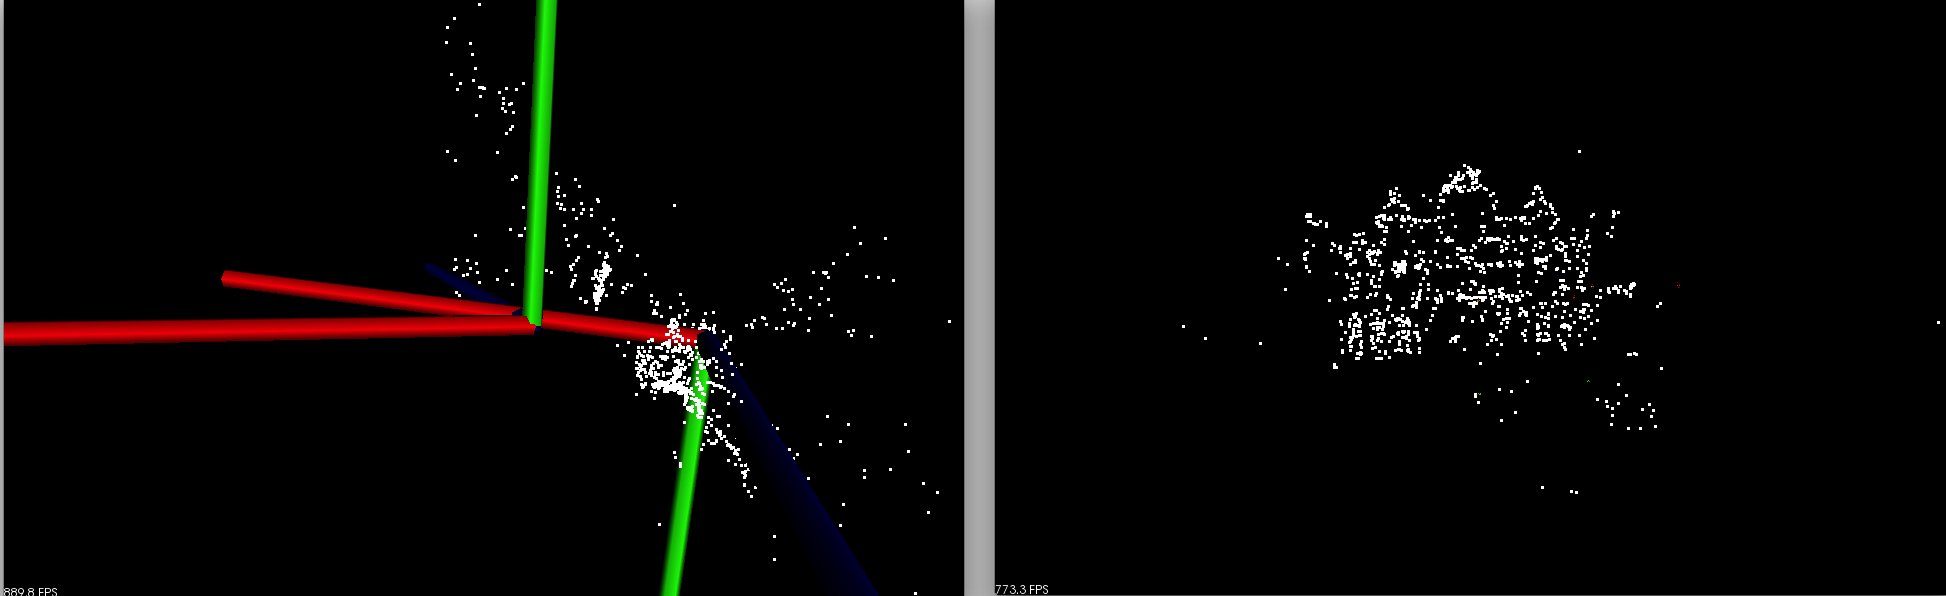
\includegraphics[width=0.9\textwidth]{FailCaseFundamental}
    \caption{Fail test case of Standard 8-point triangulation(left) in comparison to fortunate reconstruction}
    \label{fig:FailCaseFundamental}
\end{figure}
\begin{figure}[p]
    \centering
    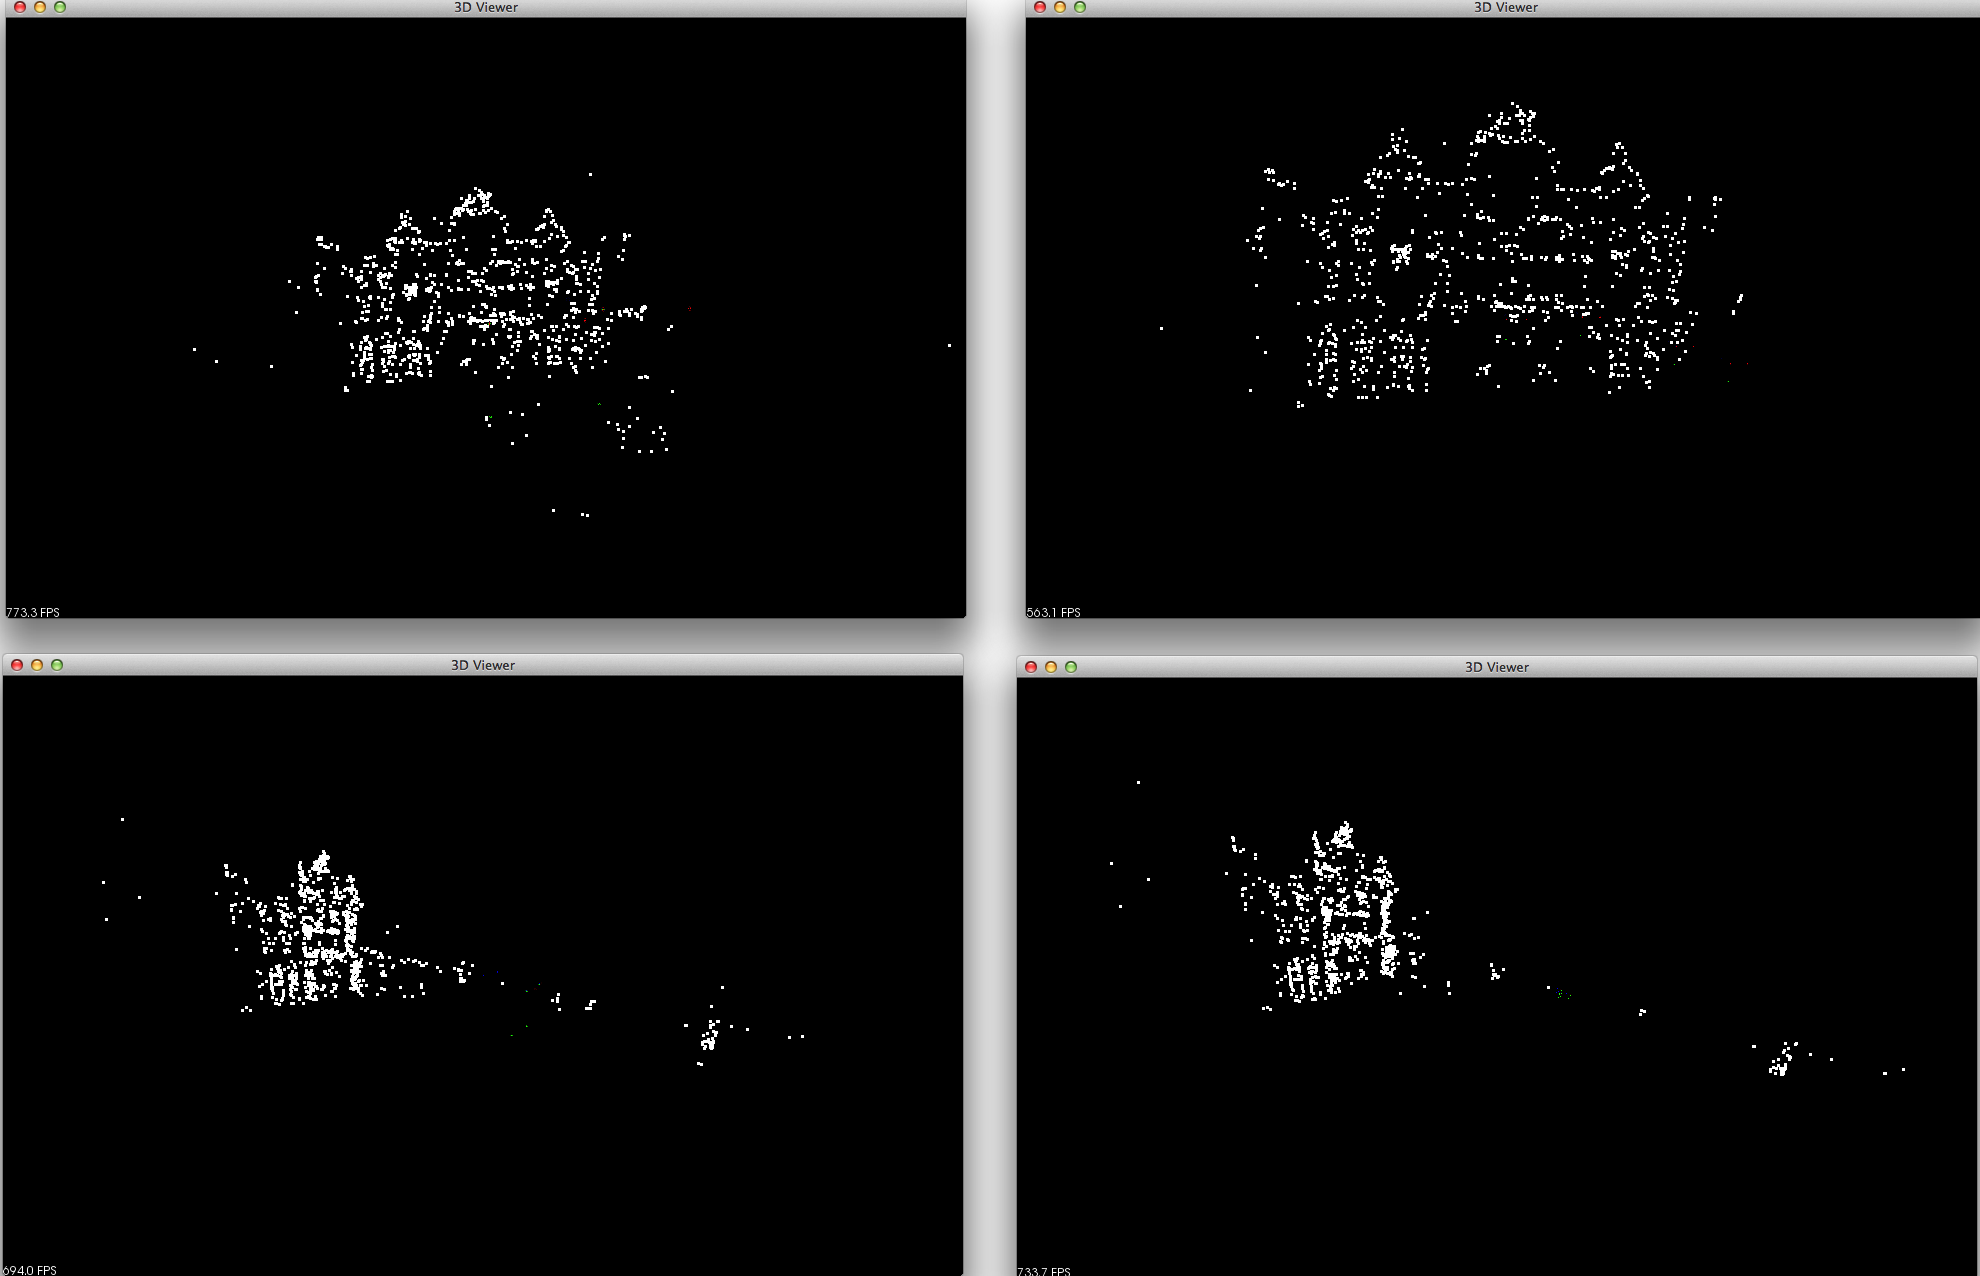
\includegraphics[width=0.9\textwidth]{PoseEstimationMethodComparison}
    \caption{Pose estimation methods comparison(Views from front and side). Left: Normal Pose Estimation, right: Enhanced Rotation and Translation Pose Estimation}. Less outliers are reconstructed when enhancment is used.
    \label{fig:PoseEstimationMethodComparison}
\end{figure}
\begin{figure}[p]
    \centering
    \includegraphics[height=18cm]{uniNone4000}
    \caption{Reconstruction results from known translations and rotations from different angles. Upper shows front face of building, other from different angles. Many outliers in reconstructed model.}
    \label{fig:UniNone4000}
\end{figure}

% ---------------------------------------------------------------------------
% ----------------------- end of thesis sub-document ------------------------
% ---------------------------------------------------------------------------

%\begin{figure}[h]
%  \begin{center}
%    \begin{tikzpicture}
%      \begin{axis}[
%          width=\linewidth, % Scale the plot to \linewidth
%          grid=major, % Display a grid
%          grid style={dashed,gray!30}, % Set the style
%          xtick = {100,500,1000,5000},
%          xlabel=Sift features number, % Set the labels
%          xmode=log,
%          log ticks with fixed point,
%          ymode=normal,
%          ylabel=Execution time(ms),
%          legend style={at={(0.5,-0.2)},anchor=north,cells={anchor=west}}, % Put the legend below the plot
%        ]
%        \addplot[mark=*,blue] table[x=Number of Sift features,y=8-pointInit+NormalPoseEstim,col sep=comma] {ReconstructInit.csv}; 
%        \addplot[mark=*,red] table[x=Number of Sift features,y=Enhanced8-point+NormalPoseEstim,col sep=comma] {ReconstructInit.csv};
%        \addplot[mark=*,orange] table[x=Number of Sift features,y=Enhanced8-point+EnhancedPoseEstim,col sep=comma] {ReconstructInit.csv}; 
%        \addplot[mark=*,pink] table[x=Number of Sift features,y=Alternative3-point+NormalPoseEstim,col sep=comma] {ReconstructInit.csv};
%        \addplot[mark=*,green] table[x=Number of Sift features,y=Alternative3-point+EnhancedPoseEstim,col sep=comma] {ReconstructInit.csv};
%        \addplot[mark=*,yellow] table[x=Number of Sift features,y=Known Rotations and Translations,col sep=comma] {ReconstructInit.csv};
%        \legend{Standard 8-point initialization + Normal OpenCV Pose Estimation,Enhanced 8-point initialization + Normal Pose Estimation,Enhanced 8-point initiazliation + Enhanced Pose Estim, Alternative 3-point initiazliation + Normal Pose Estimation, Alternative 3-point initialization + Enhanced Pose Estimation, Known Rotations and Translations}
%      \end{axis}
%    \end{tikzpicture}
%    \caption{Execution time of first pair images recontruction(1024x768pixels) in comparison to initial SIFT feature number}
%  \end{center}
%\end{figure}

% this file is called up by thesis.tex
% content in this file will be fed into the main document

\chapter{Conclusion} % top level followed by section, subsection


% ----------------------- contents from here ------------------------

\section{Summary}
\section{Dissemination}
Who uses your component or who will use it? Industry projects, EU projects, open 
source...? Is it integrated into a larger environment? Did you publish any papers? 
\section{Problems Encountered}
\section{Future work}




% ---------------------------------------------------------------------------
% ----------------------- end of thesis sub-document ------------------------
% ---------------------------------------------------------------------------              

% this file is called up by thesis.tex
% content in this file will be fed into the main document

\chapter{Materials \& methods} % top level followed by section, subsection
\begin{lstlisting}[language=json,firstnumber=1, float]
[
   {
      "photoPath":"20141210_145643/0.jpg",
      "rotationMatrix":[],
      "azimuth":121.88075,
      "posX":-1.7521392107009888,
      "posY":-1.4345977306365967,
      "posZ":0.9248641133308411,
      "photoId":1,
      "pitch":13.867888,
      "roll":178.16968
   },
   {
      "photoPath":"20141210_145643/1.jpg",
      "rotationMatrix":[],
      ],
      "azimuth":110.66925,
      "posX":-4.244707942008972,
      "posY":-1.1443554759025574,
      "posZ":0.9647054933011532,
      "photoId":2,
      "pitch":11.625216,
      "roll":179.73383
   }
   ...
]
\end{lstlisting}
\clearpage

\begin{table}[h]
\centering
\begin{adjustbox}{width=1\linewidth}
\begin{tabular}{l|l|l|l|l}
\textbf{100 SIFT Features}   & \textbf{Total Sampson Error} & \textbf{Sampson Error per Point} & \textbf{Points left} & \textbf{Execution time(ms)} \\ \hline
\textbf{8-point OpenCV}      & 20.5793             & 0.478588                & 43          & 0.4387             \\ \hline
\textbf{Alternative 3-point} & 112.749             & 4.17588                 & 27          & 0.1484             \\ \hline
\textbf{8-point enhanced}    & 67.2559             & 1.56409                 & 43          & 0.3867             \\ \hline
\textbf{Known rot and trans} & 3501.23             & 83.3625                 & 42          & 0.0001             \\ \hline
\textbf{Essential 5-point}   & 43.5866             & 1.06309                 & 41          & 0.684              \\ \hline
\textbf{5-point enhanced}    & 1863.66             & 45.4552                 & 41          & 13.4643            \\
\end{tabular}
\end{adjustbox}
\caption{Efficeincy table of proposed methods for 100 SIFT features in Warsaw Univeristy of technology dataset. Colums: Total Sampson Error, Avarage Sampson error per point, Amount of points left after outliers removal, Execution time}
\label{table:Efficiency100Sift}
\end{table}

\begin{table}[h]
\centering
\begin{adjustbox}{width=1\linewidth}
\begin{tabular}{l|l|l|l|l}
\textbf{500 SIFT features}   & \textbf{Total Sampson Error} & \textbf{Sampson Error per Point} & \textbf{Points left} \& \textbf{Execution time(ms)} \\ \hline
\textbf{8-point OpenCV}      & 100.584             & 0.543697                & 185         & 1.0833             \\ \hline
\textbf{Alternative 3-point} & 220.722             & 2.53704                 & 87          & 0.2692             \\ \hline
\textbf{8-point enhanced}    & 112.7               & 0.609189                & 185         & 0.8362             \\ \hline
\textbf{Known rot and trans} & 14770.7             & 80.2756                 & 184         & 0.0001             \\ \hline
\textbf{Essential 5-point}   & 404.098             & 2.29601                 & 176         & 3.8827             \\ \hline
\textbf{5-point enhanced}    & 501.987             & 2.8522                  & 176         & 47.0683            \\
\end{tabular}
\end{adjustbox}
\caption{Efficeincy table of proposed methods for 500 SIFT features in Warsaw Univeristy of technology dataset. Colums: Total Sampson Error, Avarage Sampson error per point, Amount of points left after outliers removal, Execution time}
\label{table:Efficiency500Sift}
\end{table}

\begin{table}[h]
\centering
\begin{adjustbox}{width=1\linewidth}
\begin{tabular}{l|l|l|l|l}
\textbf{1000 SIFT features}  & \textbf{Total Sampson Error} & \textbf{Sampson Error per Point} & \textbf{Points left} & \textbf{Execution time(ms)} \\ \hline
\textbf{8-point OpenCV}      & 265.637             & 0.781287                & 340         & 1.5055             \\ \hline
\textbf{Alternative 3-point} & 640.895             & 4.1083                  & 156         & 0.4725             \\ \hline
\textbf{8-point enhanced}    & 295.152             & 0.868093                & 340         & 1.8099             \\ \hline
\textbf{Known rot and trans} & 27394.4             & 77.1673                 & 355         & 0.0001             \\ \hline
\textbf{Essential 5-point}   & 518.293             & 1.85768                 & 279         & 5.4482             \\ \hline
\textbf{5-point enhanced}    & 349.393             & 1.2523                  & 279         & 204.2998           \\
\end{tabular}
\end{adjustbox}
\caption{Efficeincy table of proposed methods for 1000 SIFT features in Warsaw Univeristy of technology dataset. Colums: Total Sampson Error, Avarage Sampson error per point, Amount of points left after outliers removal, Execution time}
\label{table:Efficiency1000Sift}
\end{table}

\begin{table}[h]
\centering
\begin{adjustbox}{width=1\linewidth}
\begin{tabular}{l|l|l|l|l}
\textbf{5000 SIFT features}      & \textbf{Total Sampson Error} & \textbf{Sampson Error per Point} & \textbf{Points left} & \textbf{Execution time(ms)} \\ \hline
\textbf{8-point OpenCV}          & 517.189             & 0.439413                & 1177        & 2.187              \\ \hline
\textbf{Alternative 3-point}     & 1879.98             & 3.28094                 & 573         & 0.8286             \\ \hline
\textbf{8-point enhanced}        & 1087.78             & 0.924199                & 1177        & 5.4395             \\ \hline
\textbf{Known rot and trans}     & 93951.1             & 77.9677                 & 1205        & 0.0001             \\ \hline
\textbf{Essential 5-point}       & 1949.53             & 1.95736                 & 996         & 15.2223            \\ \hline
\textbf{5-point enhanced}        & 19966.6             & 20.0468                 & 996         & 355.464            \\ 
\end{tabular}
\end{adjustbox}
\caption{Efficeincy table of proposed methods for 5000 SIFT features in Warsaw Univeristy of technology dataset. Colums: Total Sampson Error, Avarage Sampson error per point, Amount of points left after outliers removal, Execution time}
\label{table:Efficiency5000Sift}
\end{table}



% ----------------------- paths to graphics ------------------------



% ----------------------- contents from here ------------------------




 

% ---------------------------------------------------------------------------
%: ----------------------- end of thesis sub-document ------------------------
% ---------------------------------------------------------------------------



 






        % description of lab methods


% --------------------------------------------------------------
%:                  BACK MATTER: appendices, refs,..
% --------------------------------------------------------------

% the back matter: appendix and references close the thesis


%: ----------------------- bibliography ------------------------

% The section below defines how references are listed and formatted
% The default below is 2 columns, small font, complete author names.
% Entries are also linked back to the page number in the text and to external URL if provided in the BibTex file.

% PhDbiblio-url2 = names small caps, title bold & hyperlinked, link to page 
%\begin{multicols}{2} % \begin{multicols}{ # columns}[ header text][ space]
\begin{footnotesize} % tiny(5) < scriptsize(7) < footnotesize(8) < small (9)

\bibliographystyle{Latex/Classes/PhDbiblio-url2} % Title is link if provided
\renewcommand{\bibname}{References} % changes the header; default: Bibliography
\nocite{*}

\bibliography{9_backmatter/references.bib} % adjust this to fit your BibTex file

\end{footnotesize}
%\end{multicols}

% --------------------------------------------------------------
% Various bibliography styles exit. Replace above style as desired.

% in-text refs: (1) (1; 2)
% ref list: alphabetical; author(s) in small caps; initials last name; page(s)
%\bibliographystyle{Latex/Classes/PhDbiblio-case} % title forced lower case
%\bibliographystyle{Latex/Classes/PhDbiblio-bold} % title as in bibtex but bold
%\bibliographystyle{Latex/Classes/PhDbiblio-url} % bold + www link if provided

%\bibliographystyle{Latex/Classes/jmb} % calls style file jmb.bst
% in-text refs: author (year) without brackets
% ref list: alphabetical; author(s) in normal font; last name, initials; page(s)

%\bibliographystyle{plainnat} % calls style file plainnat.bst
% in-text refs: author (year) without brackets
% (this works with package natbib)


% --------------------------------------------------------------

% according to Dresden med fac summary has to be at the end
%
% Thesis Abstracts -----------------------------------------------------

\selectlanguage{english}
\begin{abstract}
The main subject of this thesis addresses the possibility of enhancing the existing 3D reconstruction algorithms with additional Android sensor fusion data. The primary fundamentals behind the reconstruction techniques and the problems related to them are explained in order to introduce the reader to these topics. Related works are discussed in order to explain the strengths and weaknesses of the state-of-art reconstruction approches. The proposed enhancements using initial rotation in the standard 8-point and 5-point algorithms are explained in detail. Both of them allow for focusing on correcting rotation matrix error instead of calculating the rotation itself. This, in turn, serves for reducing ambiguity of the decomposition of essential matrix to the relative rotation and translation of the cameras. The primary idea behind the implementation of the 3-point algorithm for translation is also described. The most important aspects of the implemented $"Sensor Enhanced Image Camera"$ Android application and $"Enhanced 3D Reconstructer"$ were discussed.
The three proposed initial pair reconstruction methods were evaluated, which showed that each algorithm is able to improve certain asspects of the 3D reconstruction. Different reconstruction strategies were evaluated. As a result it was discovered that the enhanced structure computation can be faster and more accurate than the standard methodology. Using initial rotation and translation pose estimation results in significantly faster convergence and better error reduction with Bundle Adjustment. This thesis covers only some notions of the Structure from Motion, therefore plans for future development were  established.
\end{abstract}

\clearpage
\selectlanguage{ngerman} 
\begin{abstract}
Das Hauptthema dieser Arbeit befasst sich mit der M{\"o}glichkeit der Verbesserung der vorhandenen 3D-Rekonstruktionsalgorithmen mit zus{\"a}tzlichen Android Sensorfusion Daten. Die wichtigsten Grundlagen hinter den Rekonstruktionstechniken und die damit verbundenen Probleme sind, um den Leser zu diesen Themen vorstellen erl{\"a}utert. {\"A}hnliche Arbeiten sind erforderlich, um die Festigkeiten und Schw{\"a}chen der Stand-der-Technik Rekonstruktion Ansätze erkl{\"a}ren diskutiert. Die vorgeschlagenen Verbesserungen mit Anfangsrotation in den Standard 8-Punkte und 5-Punkte-Algorithmen werden im Detail erkl{\"a}rt. Beide von ihnen k{\"o}nnen zur Fokussierung auf die Rotationsmatrix Fehler Korrektur anstelle der Berechnung des Rotation selbst. Dies wiederum serviert zur Reduzierung der Mehrdeutigkeit des Essential-Matrix Zersetzungs zu der relativen Rotation und Translation den Kameras. Die Hauptidee hinter der Umsetzung der 3-Punkt-Algorithmus f{\"u}r die Translation ist ebenfalls beschrieben. Die wichtigsten Aspekte die implementierten $"Sensor Verbesserte Bildkamera "$ Android-Anwendung und $ "Verbesserte 3D Reconstructer "$  wurden diskutiert.
Die drei vorgeschlagenen ersten Paar Rekonstruktionsmethoden wurden bewertet, die zeigten, dass jeder Algorithmus kann bestimmte asspects der 3D-Rekonstruktion zu verbessern. Verschiedene Rekonstruktionsstrategien wurden bewertet. Als Ergebnis wurde festgestellt, dass die verbesserte Struktur Berechnung kann schneller und genauer als die Standardmethode sein. Mit  anfänglichen Rotation und Translation  Posenschätzung resultiert in signifikant schneller Konvergenz und besseres Fehlerreduktion mit B{\"u}ndelausgleichung. Diese Diplomarbeit umfasst nur einige Vorstellungen von der Struktur aus Bewegung, daher plant f{\"u}r die zuk{\"u}nftige Entwicklung entstanden.
\end{abstract}
\selectlanguage{english}

%: Declaration of originality

% Thesis statement of originality -------------------------------------

% Depending on the regulations of your faculty you may need a declaration like the one below. This specific one is from the medical faculty of the university of Dresden.

\begin{declaration}        %this creates the heading for the declaration page

I herewith declare that I have produced this paper without the prohibited assistance of third parties and without making use of aids other than those specified; notions taken over directly or indirectly from other sources have been identified as such. This paper has not previously been presented in identical or similar form to any other German or foreign examination board.

The thesis work was conducted from XXX to YYY under the supervision of PI at ZZZ.

\vspace{10mm}

CITY,


\end{declaration}


% ----------------------------------------------------------------------



\end{document}
